\appendix

\chapter{Examples}
\label{Examples}

%In this chapter, we report code of the \textsc{Line} examples under the \texttt{examples/} folder and their outputs.
\Matlab{The table below lists the scripts available under the \texttt{examples/} folder.}
\Java{The table below lists the examples available under the \texttt{Examples} package.}
\Python{The table below lists the Jupyter notebooks available under the \texttt{examples/} folder.}
\begin{footnotesize}
\begin{longtable}{|p{0.35\linewidth}|p{0.60\linewidth}|}
\caption{Examples}
\\\hline
\textbf{Example} & \textbf{Problem}
\\\hline
\endfirsthead
\multicolumn{2}{c}%
{\tablename\ \thetable\ -- Examples.\textit{ Continued from previous page}} \\
\hline
\textbf{Example} & \textbf{Problem}\\
\hline
\endhead
\hline \multicolumn{2}{r}{\textit{Continued on next page}} \\
\endfoot
\hline
\endlastfoot
%\texttt{example\_BPMN\_1} &  Example of model-to-model transformation from BPMN to Layered network\\
%\texttt{example\_BPMN\_2} &  Example of model-to-model transformation from BPMN to Layered network\\
\hline
\texttt{ag\_closed\_network} & Closed network agent model\\
\texttt{ag\_jackson\_network} & Jackson network agent model\\
\texttt{ag\_multiclass\_closed} & Multiclass closed agent model\\
\texttt{ag\_tandem\_open} & Open tandem agent model\\
\hline
\texttt{cache\_replc\_rr} &  A small cache model with an open arrival process\\
\texttt{cache\_replc\_fifo} &  A small cache model with a closed job population\\
\texttt{cache\_replc\_lru} &  A layered network with a caching layer\\
\texttt{cache\_compare\_replc} &  A layered network with a caching layer having a multi-level cache\\
\texttt{cache\_replc\_routing} &  A caching model with state-dependent output routing\\
\hline
\texttt{cdf\_respt\_closed} &  Station response time distribution in a single-class single-job closed network\\
\texttt{cdf\_respt\_closed\_threeclasses} &  Station response time distribution in a multi-chain closed network\\
\texttt{cdf\_respt\_open\_twoclasses} &  Station response time distribution in a multi-chain open network\\
\texttt{cdf\_respt\_distrib} &  Simulation-based station response time distribution analysis\\
\texttt{cdf\_respt\_populations} &  Station response time distribution under increasing job populations\\
\hline
\texttt{fcr\_lossn} & Loss network analysis using finite capacity regions\\
\hline
\texttt{cqn\_repairmen} &  Solving a single-class exponential closed queueing network\\
\texttt{cqn\_twoclass\_hyperl} &  Solving a closed queueing network with a multi-class FCFS station\\
\texttt{cqn\_threeclass\_hyperl} &  Solving exactly a multi-chain product-form closed queueing network\\
\texttt{cqn\_multiserver} &  Local state space generation for a station in a closed network\\
\texttt{cqn\_oneline} &  1-line exact MVA solution of a cyclic network of PS and INF stations\\
\texttt{cqn\_twoclass\_erl} &  Closed network with round robin scheduling\\
\texttt{cqn\_bcmp\_theorem} &  Comparison of different scheduling policies that preserve the product-form solution\\
\texttt{cqn\_repairmen\_multi} &  Multi-server closed queueing network with repairmen\\
\texttt{cqn\_twoqueues\_multi} &  Closed queueing network with two multi-server queues\\
\texttt{cqn\_twoqueues} &  Simple closed network with two queues\\
\hline
\texttt{cs\_implicit} &  Class switching with implicit routing\\
\texttt{cs\_multi\_diamond} & Class switching with multiple diamond patterns\\
\texttt{cs\_single\_diamond} & Class switching with single diamond pattern\\
\texttt{cs\_transient\_class} & Class switching with transient classes\\
\hline
\texttt{fj\_basic\_open} & A simple single class open fork-join network\\
\texttt{fj\_twoclasses\_forked} & A multiclass open fork-join network\\
\texttt{fj\_basic\_nesting} & A closed model with nested forks and joins\\
\texttt{fj\_nojoin} & An open model with a fork but without a join\\
\texttt{fj\_basic\_closed} & A simple single class closed fork-join network\\
\texttt{fj\_serialfjs\_open} & Two open fork-joins subsystems in tandem\\
\texttt{fj\_cs\_postfork} & Two-class fork-join with a class that switches into the other after the fork\\
\texttt{fj\_cs\_multi\_visits} & Two fork-joins loops within the same chain\\
\texttt{fj\_route\_overlap} & A model with overlapping routes in a fork-join network\\
\texttt{fj\_asymm} & Asymmetric fork-join network\\
\texttt{fj\_delays} & Fork-join network with delays\\
\texttt{fj\_complex\_serial} & Complex serial fork-join network\\
\texttt{fj\_threebranches} & Fork-join network with three branches\\
\texttt{fj\_cs\_prefork} & Fork-join network with class-switching before fork\\
\texttt{fj\_deep\_nesting} & Fork-join network with deep nesting\\
\texttt{fj\_serialfjs\_closed} & Closed serial fork-join network\\
\hline
\texttt{init\_state\_fcfs\_exp} &  Specifying an initial state and prior in a single class model.\\
\texttt{init\_state\_fcfs\_nonexp} &  Specifying an initial state and prior in a multiclass model.\\
\texttt{init\_state\_ps} &  Specifying an initial state and prior in a model with class-switching.\\
\hline
\texttt{lqn\_serial} & Analyze a layered network specified in a LQNS XML file \\
\texttt{lqn\_multi\_solvers} & Specifying and solving a basic layered network\\
\texttt{lqn\_init} & Specifying and solving a basic layered network with initialization\\
\texttt{lqn\_twotasks} & Layered network with two tasks\\
\texttt{lqn\_bpmn} & BPMN to layered network transformation\\
\texttt{lqn\_workflows} & Workflow modeling in layered networks\\
\texttt{lqn\_function} & Layered network function modeling\\
\texttt{lqn\_basic} & Basic layered network example\\
%\texttt{example\_layeredModel\_3} & Specifying and solving a basic layered network\\
%\texttt{example\_layeredModel\_4} & Specifying and solving a basic layered network\\
%\texttt{example\_layeredModel\_5} & Specifying and solving a basic layered network\\
%\texttt{example\_layeredModel\_6} & Specifying and solving a basic layered network\\
%\texttt{example\_layeredModel\_7} & Specifying and solving a basic layered network\\
\hline
\texttt{ld\_multiserver\_fcfs} &  Solving a single-class load-dependent closed model\\
\texttt{ld\_multiserver\_ps\_twoclasses} &  Solving a two-node multiclass load-dependent closed model\\
\texttt{ld\_multiserver\_ps} &  Solving a three-node multiclass load-dependent closed model\\
\texttt{ld\_class\_dependence} &  Load-dependent model with class dependence\\
\hline
\texttt{cqn\_scheduling\_dps} &  Parameterization of a discriminatory processor sharing (DPS) station\\
\texttt{cqn\_mmpp2\_service} &  Automatic detection of solvers that cannot analyze the model\\
\hline
\texttt{mqn\_basic} & Solving a queueing network model with both closed and open classes \\
\texttt{mqn\_multiserver\_ps} & A difficult mixed model with sparse routing among multi-server nodes \\
\texttt{mqn\_multiserver\_fcfs} & Mixed model with multiserver FCFS nodes\\
\texttt{mqn\_singleserver\_fcfs} & Mixed model with single server FCFS\\
\texttt{mqn\_singleserver\_ps} & Mixed model with single server PS\\
\hline
\texttt{oqn\_basic} & Solving a queueing network model with open classes, scalar cutoff options \\
\texttt{oqn\_oneline} & 1-line solution of a tandem network of PS and INF stations\\
\texttt{oqn\_cs\_routing} & Solving a queueing network model with open classes, matrix cutoff options \\
\texttt{oqn\_trace\_driven} & Trace-driven simulation of an M/M/1 queue\\
\texttt{oqn\_vsinks} & A model illustrating the emulation of multiple sinks\\
\texttt{oqn\_fourqueues} & A large multiclass example with PS and FCFS\\
\hline
\texttt{prio\_hol\_open} & A multiclass example with PS, SIRO, FCFS, FCFSPRIO priority\\
\texttt{prio\_hol\_closed} & A high-load multiclass example with PS, SIRO, FCFS, FCFSPRIO priority\\
\texttt{prio\_psprio} & A repaimen model with PS priority scheduling. \\
\texttt{prio\_identical} & Priority model with identical classes\\
\hline
\texttt{renv\_twostages\_repairmen} &  Solving a model in a 2-stage random environment with exponential rates\\
\texttt{renv\_fourstages\_repairmen} &  Solving a model in a 4-stage random environment with Coxian rates \\
\texttt{renv\_threestages\_repairmen} &  Solving a model in a 3-stage random environment with Erlang rates\\
\texttt{renv\_node\_breakdown} &  Using simplified breakdown/repair API for node failures in random environments\\
\texttt{renv\_node\_breakdown\_example} &  Using simplified breakdown/repair API for node failures in random environments\\
\hline
\texttt{example\_rewardModel\_1} &  Reward-based CTMC analysis using custom reward functions (setReward, getReward, getAvgReward)\\
\hline
\texttt{sdroute\_closed} & A model with round-robin routing \\
\texttt{sdroute\_twoclasses\_closed} & A model with round-robin routing after multi-class PH and MAP service\\
\texttt{sdroute\_open} & A load-balancer modeled as a router\\
\hline
\texttt{statepr\_aggr} &  Computing marginal state probabilities for a node\\
\texttt{statepr\_aggr\_large} &  Computing marginal state probabilities for a node under class-switching\\
\texttt{statepr\_sys\_aggr} &  Computing joint state probabilities for a system with two nodes under class-switching\\
\texttt{statepr\_sys\_aggr\_large} &  Computing joint state probabilities under class-switching and with delay nodes\\
\texttt{statepr\_allprobs\_ps} &  Computing probabilities under PS class-switching and with delay nodes\\
\texttt{statepr\_allprobs\_fcfs} &  Computing  probabilities under PS and FCFS class-switching and with delay nodes\\
\hline
\texttt{spn\_basic\_open} &  JMT simulation of a simple stochastic Petri net model\\
\texttt{spn\_open\_sevenplaces} &  JMT simulation of a complex stochastic Petri net model\\
\texttt{spn\_twomodes} & Stochastic Petri net with two modes\\
\texttt{spn\_fourmodes} & Stochastic Petri net with four modes\\
\texttt{spn\_inhibiting} & Stochastic Petri net with inhibiting transitions\\
\texttt{spn\_closed\_fourplaces} & Closed Stochastic Petri net with four places\\
\texttt{spn\_closed\_twoplaces} & Closed Stochastic Petri net with two places\\
\texttt{spn\_basic\_closed} & Basic closed stochastic Petri net\\
\hline
\texttt{tut01\_mm1\_basics} & M/M/1 queue basics\\
\texttt{tut02\_mg1\_multiclass\_solvers} & M/G/1 multiclass solvers\\
\texttt{tut03\_repairmen} & Repairmen model\\
\texttt{tut04\_lb\_routing} & Load balancing routing\\
\texttt{tut05\_completes\_flag} & Complete flag usage\\
\texttt{tut06\_cache\_lru\_zipf} & Cache LRU Zipf distribution\\
\texttt{tut07\_respt\_cdf} & Response time CDF analysis\\
\texttt{tut08\_opt\_load\_balancing} & Optimal load balancing\\
\texttt{tut09\_dep\_process\_analysis} & Dependent process analysis\\
\texttt{tut10\_lqn\_basics} & Layered queueing network basics\\
\texttt{tut12\_posterior\_analysis} & Posterior analysis and parameter inference\\
\hline
\texttt{lcq\_singlehost} & Single host layered cache queueing\\
\texttt{lcq\_threehosts} & Three hosts layered cache queueing\\
\hline
\texttt{swt\_basic} & Basic switchover times model\\
\hline
\texttt{polling\_exhaustive\_exp} & Exhaustive polling with exponential times\\
\texttt{polling\_gated} & Gated polling\\
\texttt{polling\_klimited} & K-limited polling\\
\texttt{polling\_exhaustive\_det} & Exhaustive polling with deterministic times\\
% \hline
% \texttt{example\_scvEstimation\_1} &  Demand estimation in a single class model using the UBR method\\
% \texttt{example\_scvEstimation\_2} &  Demand estimation in a multiclass model using the ERPS method\\
% \texttt{example\_scvEstimation\_3} &  Demand estimation in a multiclass model using the UBR method\\
% \texttt{example\_scvEstimation\_4} &  Demand estimation in a multiclass model using the UBO method%\\
\label{TAB_examples_closedModel}
\end{longtable}
\end{footnotesize}

%\subsection{\texttt{cqn\_repairmen.m}}
%\paragraph{Code.} This example illustrates the definition in \textsc{Line} of a single-class closed queueing network with two nodes,a  delay and a processor sharing queue, and probabilistic routing. All available \textsc{Line} solvers are instantiated and run on the model.
%%\lstinputlisting[language=matlab,numbers=left,linerange=1-27]{examples/cqn_repairmen.m}
%
%\lstset{
%    language=matlab,
%    tabsize=3,
%    frame=single,
%    basicstyle=\ttfamily\scriptsize,
%    %caption=Test,
%    label=code:sample,
%    frame=shadowbox,
%    rulesepcolor=\color{gray},
%    xleftmargin=20pt,
%    framexleftmargin=15pt,
%    keywordstyle=\color{black},
%    commentstyle=\color{magenta},
%    stringstyle=\color{red},
%    %numbers=left,
%    %numberstyle=\tiny,
%    %numbersep=5pt,
%    aboveskip=10pt,
%    breaklines=true,
%    showstringspaces=false,
%    emph={environment,stage,envParameter,coxDistribution,coxParameter},
%    emphstyle={\color{blue}}}
%
%\begin{lstlisting}
%clear;
%model = Network('model');
%
%node{1} = Delay(model, 'Delay');
%node{2} = Queue(model, 'Queue1', SchedStrategy.PS);
%jobclass{1} = ClosedClass(model, 'Class1', 5, node{1}, 0);
%
%node{1}.setService(jobclass{1}, Exp.fitMeanAndSCV(1.0)); % mean = 1
%node{2}.setService(jobclass{1}, Exp.fitMeanAndSCV(2.0)); % mean = 2
%
%model.addLink(node{1}, node{1});
%model.addLink(node{1}, node{2});
%model.addLink(node{2}, node{1});
%model.addLink(node{2}, node{2});
%
%node{1}.setProbRouting(jobclass{1}, node{1}, 0.7)
%node{1}.setProbRouting(jobclass{1}, node{2}, 0.3)
%node{2}.setProbRouting(jobclass{1}, node{1}, 1.0)
%
%solver = {};
%solver{end+1} = CTMC(model);
%solver{end+1} = JMT(model);
%solver{end+1} = SSA(model);
%solver{end+1} = FLD(model);
%solver{end+1} = MVA(model);
%solver{end+1} = NC(model);
%for s=1:length(solver)
%    fprintf(1,'SOLVER: %s\n',solver{s}.getName());
%    AvgTable = solver{s}.getAvgTable()
%end
%\end{lstlisting}
%
%\paragraph{Output.} The output of the previous script is as follows. Small approximation errors and simulation sampling error are responsible from small deviations from the exact values, which are those reported by the CTMC solver. The error of the simulation solvers (JMT, SSA) can be increase with larger \texttt{options.samples} values.
%
%\begin{lstlisting}
%SOLVER: CTMC
%AvgTable =
%  2x6 table
%    Station         Class          QLen      Util      RespT      Tput
%    ________    ______________    ______    _______    ______    ______
%    'Delay'     'Class1'    1.6327     1.6327         1    1.6327
%    'Queue1'    'Class1'    3.3673    0.97961    6.8748    0.4898
%SOLVER: JMT
%AvgTable =
%  2x6 table
%    Station         Class          QLen      Util      RespT      Tput
%    ________    ______________    ______    _______    ______    _______
%    'Delay'     'Class1'    1.5491     1.5491    1.0042     1.6093
%    'Queue1'    'Class1'      3.39    0.98315     6.967    0.48154
%SOLVER: SSA
%AvgTable =
%  2x6 table
%    Station         Class          QLen      Util      RespT      Tput
%    ________    ______________    ______    _______    ______    _______
%    'Delay'     'Class1'    1.6309     1.6309         1     1.6309
%    'Queue1'    'Class1'    3.3691    0.97853    6.8694    0.49045
%SOLVER: FLD
%AvgTable =
%  2x6 table
%    Station      Class       QLen      Util     RespT      Tput
%    ________    ________    ______    ______    ______    ______
%    'Delay'     'Class1'    1.6667    1.6667         1    1.6667
%    'Queue1'    'Class1'    3.3333         1    6.6667       0.5
%SOLVER: MVA
%AvgTable =
%  2x6 table
%    Station         Class          QLen      Util      RespT      Tput
%    ________    ______________    ______    _______    ______    _______
%    'Delay'     'Class1'    1.5314     1.5314         1     1.5314
%    'Queue1'    'Class1'    3.4686    0.91886    7.5497    0.45943
%SOLVER: NC
%AvgTable =
%  2x6 table
%    Station         Class          QLen      Util      RespT      Tput
%    ________    ______________    ______    _______    ______    ______
%    'Delay'     'Class1'    1.6327     1.6327         1    1.6327
%    'Queue1'    'Class1'    3.3673    0.97961    6.8748    0.4898
%\end{lstlisting}
%
%\subsection{\texttt{example\_closedModel\_2.m}}
%\paragraph{Code.}  This model shows an example of 2-class, 1-chain, closed queueing network with non-exponential service processes.
%\begin{lstlisting}
%model = Network('model');
%
%node{1} = Delay(model, 'Delay');
%node{2} = Queue(model, 'Queue1', SchedStrategy.FCFS);
%node{2}.setNumServers(2);
%
%jobclass{1} = ClosedClass(model, 'Class1', 2, node{1}, 0);
%jobclass{2} = ClosedClass(model, 'Class2', 2, node{1}, 0);
%
%node{1}.setService(jobclass{1}, Erlang(3,2));
%node{1}.setService(jobclass{2}, HyperExp(0.5,3.0,10.0));
%
%node{2}.setService(jobclass{1}, HyperExp(0.1,1.0,10.0));
%node{2}.setService(jobclass{2}, Exp(1));
%
%M = model.getNumberOfStations();
%K = model.getNumberOfClasses();
%
%P = cell(K,K);
%P{1,1} = [0.3,0.1; 0.2,0];
%P{1,2} = [0.6,0; 0.8,0];
%P{2,2} = [0,1; 0,0];
%P{2,1} = [0,0; 1,0];
%
%model.link(P);
%
%options = Solver.defaultOptions;
%options.keep=true;
%options.verbose=1;
%options.samples=5e3;
%
%solver={};
%solver{end+1} = CTMC(model,options);
%solver{end+1} = JMT(model,options);
%solver{end+1} = SSA(model,options);
%solver{end+1} = FLD(model,options);
%solver{end+1} = MVA(model,options);
%solver{end+1} = NC(model,options);
%for s=1:length(solver)
%    fprintf(1,'SOLVER: %s\n',solver{s}.getName());
%    AvgTable = solver{s}.getAvgTable()
%end
%\end{lstlisting}
%\paragraph{Output.}
%\begin{lstlisting}
%SOLVER: CTMC
%CTMC generator and state space saved in: C:\X\AppData\Local\Temp\tp49e94d44_0a44_4d6f_ac03_68e9bb550698.mat
%CTMC analysis completed in 0.940576 sec
%AvgTable =
%  4x6 table
%    Station         Class          QLen        Util       RespT      Tput
%    ________    ______________    _______    ________    _______    _______
%    'Delay'     'Class1'     1.5404      1.5404    0.66667     2.3107
%    'Delay'     'Class2'    0.34044     0.34044    0.21667     1.5712
%    'Queue1'    'Class1'    0.11129    0.021951    0.48165    0.23107
%    'Queue1'    'Class2'     2.0078     0.78562     1.2779     1.5712
%SOLVER: JMT
%JMT Model: C:\X\AppData\Local\Temp\jsimg\tpf370d5af_7e96_4aca_bf73_0cf3c496ad2c.jsimg
%JMT Command: java -cp "C:\X\Dropbox\code\line-solver.git\bin\line\src\solvers\JMT\JMT.jar" jmt.commandline.Jmt sim "C:\X\AppData\Local\Temp\jsimg\tpf370d5af_7e96_4aca_bf73_0cf3c496ad2c.jsimg" -seed 23000 --illegal-access=permit
%JMT analysis completed in 17.300090 sec
%AvgTable =
%  4x6 table
%    Station         Class          QLen        Util       RespT      Tput
%    ________    ______________    _______    ________    _______    _______
%    'Delay'     'Class1'     1.6167      1.6167    0.65263     2.3886
%    'Delay'     'Class2'     0.3398      0.3398     0.2185     1.6104
%    'Queue1'    'Class1'    0.10854    0.018798    0.47573    0.23014
%    'Queue1'    'Class2'     1.9709     0.79182     1.2305     1.6049
%SOLVER: SSA
%SSA samples:   5000
%SSA analysis completed in 19.095364 sec
%AvgTable =
%  4x6 table
%    Station         Class          QLen        Util       RespT      Tput
%    ________    ______________    _______    ________    _______    ______
%    'Delay'     'Class1'     1.5162      1.5162    0.64725    2.3425
%    'Delay'     'Class2'    0.32429     0.32429     0.2142     1.514
%    'Queue1'    'Class1'    0.09591    0.022254     0.4954    0.1936
%    'Queue1'    'Class2'     2.0636     0.75698     1.2922     1.597
%SOLVER: FLD
%Fluid analysis completed in 0.144978 sec [21 iterations]
%AvgTable =
%  4x6 table
%    Station         Class           QLen        Util       RespT      Tput
%    ________    ______________    ________    ________    _______    _______
%    'Delay'     'Class1'      1.7625      1.7625    0.66667     2.6438
%    'Delay'     'Class2'     0.38951     0.38951    0.21667     1.7978
%    'Queue1'    'Class1'    0.050231    0.025116       0.19    0.26438
%    'Queue1'    'Class2'      1.7978     0.89888          1     1.7978
%SOLVER: MVA
%MVA analysis completed in 0.051836 sec
%AvgTable =
%  4x6 table
%    Station         Class           QLen        Util       RespT      Tput
%    ________    ______________    ________    ________    _______    _______
%    'Delay'     'Class1'      1.5557      1.5557    0.66667     2.3336
%    'Delay'     'Class2'     0.34382     0.34382    0.21667     1.5868
%    'Queue1'    'Class1'    0.057094    0.022169    0.24466    0.23336
%    'Queue1'    'Class2'      2.0434     0.79342     1.2877     1.5868
%SOLVER: NC
%NC analysis completed in 0.002516 sec
%AvgTable =
%  4x6 table
%    Station      Class        QLen       Util       RespT      Tput
%    ________    _________    _______    _______    _______    _______
%    'Delay'     'Class1'     1.0825     1.0825    0.66667     1.6237
%    'Delay'     'Class2'    0.23922    0.23922    0.21667     1.1041
%    'Queue1'    'Class1'    0.34337    0.12016     2.1148    0.16237
%    'Queue1'    'Class2'     2.3349    0.81706     2.1148     1.1041
%\end{lstlisting}
%
%\subsection{\texttt{example\_closedModel\_3.m}}
%\paragraph{Code.} This model shows an example of 3-class, 2-chain, closed queueing network with non-exponential service processes.
%\begin{lstlisting}
%model = Network('model');
%
%node{1} = Delay(model, 'Delay');
%node{2} = Queue(model, 'Queue1', SchedStrategy.PS);
%
%jobclass{1} = ClosedClass(model, 'Class1', 2, node{1}, 0);
%jobclass{2} = ClosedClass(model, 'Class2', 0, node{1}, 0);
%jobclass{3} = ClosedClass(model, 'Class3', 1, node{1}, 0);
%
%node{1}.setService(jobclass{1}, Erlang(3,2));
%node{1}.setService(jobclass{2}, HyperExp(0.5,3.0,10.0));
%node{1}.setService(jobclass{3}, Exp(1));
%
%node{2}.setService(jobclass{1}, HyperExp(0.1,1.0,10.0));
%node{2}.setService(jobclass{2}, Exp(2));
%node{2}.setService(jobclass{3}, Exp(3));
%
%M = model.getNumberOfStations();
%K = model.getNumberOfClasses();
%
%P = cell(K,K);
%
%P{1,1} = [0.3,0.1; 0.2,0];
%P{1,2} = [0.6,0; 0.8,0];
%P{1,3} = zeros(M);
%
%P{2,1} = [0,0; 1,0];
%P{2,2} = [0,1; 0,0];
%P{2,3} = zeros(M);
%
%P{3,1} = zeros(M);
%P{3,2} = zeros(M);
%P{3,3} = circul(M);
%
%model.link(P);
%
%options = Solver.defaultOptions;
%options.keep=true;
%options.verbose=1;
%
%solver={};
%solver{end+1} = CTMC(model,options);
%solver{end+1} = FLD(model,options);
%solver{end+1} = MVA(model,options);
%solver{end+1} = NC(model,options);
%for s=1:length(solver)
%    fprintf(1,'SOLVER: %s\n',solver{s}.getName());
%    AvgTable = solver{s}.getAvgTable()
%    AvgChainTable = solver{s}.getAvgChainTable()
%    AvgSysChainTable = solver{s}.getAvgSysTable()
%end
%\end{lstlisting}
%\paragraph{Output.} This is the output on screen of this example.
%\begin{lstlisting}
%SOLVER: CTMC
%CTMC generator and state space saved in: C:\X\AppData\Local\Temp\tpafad0e65_193e_4a46_a779_b2ac27a9f97f.mat
%CTMC analysis completed in 0.168026 sec
%AvgTable =
%  6x6 table
%    Station         Class     QLen        Util       RespT      Tput
%    ________    _________    ________    ________    _______    _______
%    'Delay'     'Class1'     0.94598     0.94598    0.66667      1.419
%    'Delay'     'Class2'     0.20906     0.20906    0.21667     0.9649
%    'Delay'     'Class3'     0.63412     0.63412          1    0.63412
%    'Queue1'    'Class1'    0.044719    0.026961    0.31515     0.1419
%    'Queue1'    'Class2'     0.80023     0.48245    0.82934     0.9649
%    'Queue1'    'Class3'     0.36588     0.21137    0.57699    0.63412
%AvgChainTable =
%  4x7 table
%    Station      Chain       Classes       QLen       Util       RespT      Tput
%    ________    ________    __________    _______    _______    _______    _______
%    'Delay'     'Chain1'    {1x2 cell}      1.155      1.155    0.48452     2.3839
%    'Delay'     'Chain2'    {1x1 cell}    0.63412    0.63412          1    0.63412
%    'Queue1'    'Chain1'    {1x2 cell}    0.84495    0.50941    0.35444     1.1068
%    'Queue1'    'Chain2'    {1x1 cell}    0.36588    0.21137    0.57699    0.63412
%AvgSysChainTable =
%  2x4 table
%     Chain       Classes      SysRespT    SysTput
%    ________    __________    ________    _______
%    'Chain1'    {1x2 cell}    0.83897      2.3839
%    'Chain2'    {1x1 cell}      1.577     0.63412
%SOLVER: FLD
%Fluid analysis completed in 0.059826 sec [1 iterations]
%AvgTable =
%  6x6 table
%    Station         Class     QLen        Util       RespT      Tput
%    ________    ________    ________    ________    _______    ______
%    'Delay'     'Class1'      1.1367      1.1367    0.66667     1.705
%    'Delay'     'Class2'     0.25121     0.25121    0.21667    1.1594
%    'Delay'     'Class3'        0.75        0.75          1      0.75
%    'Queue1'    'Class1'    0.032396    0.032396       0.19    0.1705
%    'Queue1'    'Class2'     0.57971     0.57971        0.5    1.1594
%    'Queue1'    'Class3'        0.25        0.25    0.33333      0.75
%AvgChainTable =
%  4x7 table
%    Station      Chain       Classes       QLen       Util       RespT      Tput
%    ________    ________    __________    _______    _______    _______    ______
%    'Delay'     'Chain1'    {1x2 cell}     1.3879     1.3879    0.48452    2.8645
%    'Delay'     'Chain2'    {1x1 cell}       0.75       0.75          1      0.75
%    'Queue1'    'Chain1'    {1x2 cell}    0.61211    0.61211    0.21369    1.3299
%    'Queue1'    'Chain2'    {1x1 cell}       0.25       0.25    0.33333      0.75
%AvgSysChainTable =
%  2x4 table
%     Chain       Classes      SysRespT    SysTput
%    ________    __________    ________    _______
%    'Chain1'    {1x2 cell}    0.69821     2.8645
%    'Chain2'    {1x1 cell}     1.3333       0.75
%SOLVER: MVA
%MVA analysis completed in 0.029756 sec
%AvgTable =
%  6x6 table
%    Station      Class       QLen        Util       RespT      Tput
%    ________    _________   ________    ________    _______    _______
%    'Delay'     'Class1'     0.90548     0.90548    0.66667     1.3582
%    'Delay'     'Class2'     0.20011     0.20011    0.21667    0.92359
%    'Delay'     'Class3'     0.61295     0.61295          1    0.61295
%    'Queue1'    'Class1'    0.047336    0.025806    0.34851    0.13582
%    'Queue1'    'Class2'     0.84707      0.4618    0.91714    0.92359
%    'Queue1'    'Class3'     0.38705     0.20432    0.63147    0.61295
%AvgChainTable =
%  4x7 table
%    Station      Chain       Classes       QLen       Util       RespT      Tput
%    ________    ________    __________    _______    _______    _______    _______
%    'Delay'     'Chain1'    {1x2 cell}     1.1056     1.1056    0.48452     2.2818
%    'Delay'     'Chain2'    {1x1 cell}    0.61295    0.61295          1    0.61295
%    'Queue1'    'Chain1'    {1x2 cell}     0.8944     0.4876    0.39197     1.0594
%    'Queue1'    'Chain2'    {1x1 cell}    0.38705    0.20432    0.63147    0.61295
%AvgSysChainTable =
%  2x4 table
%     Chain       Classes      SysRespT    SysTput
%    ________    __________    ________    _______
%    'Chain1'    {1x2 cell}    0.87649      2.2818
%    'Chain2'    {1x1 cell}     1.6315     0.61295
%SOLVER: NC
%NC analysis completed in 0.044545 sec
%AvgTable =
%  6x6 table
%    Station      Class        QLen       Util        RespT       Tput
%    ________    ________    ________    _______    _________    _______
%    'Delay'     'Class1'      252.34     252.34      0.66667     378.51
%    'Delay'     'Class2'      55.766     55.766      0.21667     257.38
%    'Delay'     'Class3'     0.63412    0.63412            1    0.63412
%    'Queue1'    'Class1'    0.044719     7.1916    0.0011815     37.851
%    'Queue1'    'Class2'     0.80023     128.69    0.0031091     257.38
%    'Queue1'    'Class3'     0.36588    0.21137      0.57699    0.63412
%AvgChainTable =
%  4x7 table
%    Station      Chain       Classes       QLen       Util        RespT       Tput
%    ________    ________    __________    _______    _______    _________    _______
%    'Delay'     'Chain1'    {1x2 cell}      308.1      308.1      0.48452     635.89
%    'Delay'     'Chain2'    {1x1 cell}    0.63412    0.63412            1    0.63412
%    'Queue1'    'Chain1'    {1x2 cell}    0.84495     135.88    0.0013288     295.23
%    'Queue1'    'Chain2'    {1x1 cell}    0.36588    0.21137      0.57699    0.63412
%AvgSysChainTable =
%  2x4 table
%     Chain       Classes      SysRespT     SysTput
%    ________    __________    _________    _______
%    'Chain1'    {1x2 cell}    0.0031452     635.89
%    'Chain2'    {1x1 cell}        1.577    0.63412
%\end{lstlisting}


\begin{comment}
\chapter{Class hierarchy}
\label{classhierarchy}
\section{Top-level classes}
\textsc{Line} uses a hierarchy of over 100 classes, all inheriting from the default \texttt{handle} class available both in MATLAB and Octave.
The top-level classes are shown in the next diagram:
\begin{center}
{\tiny
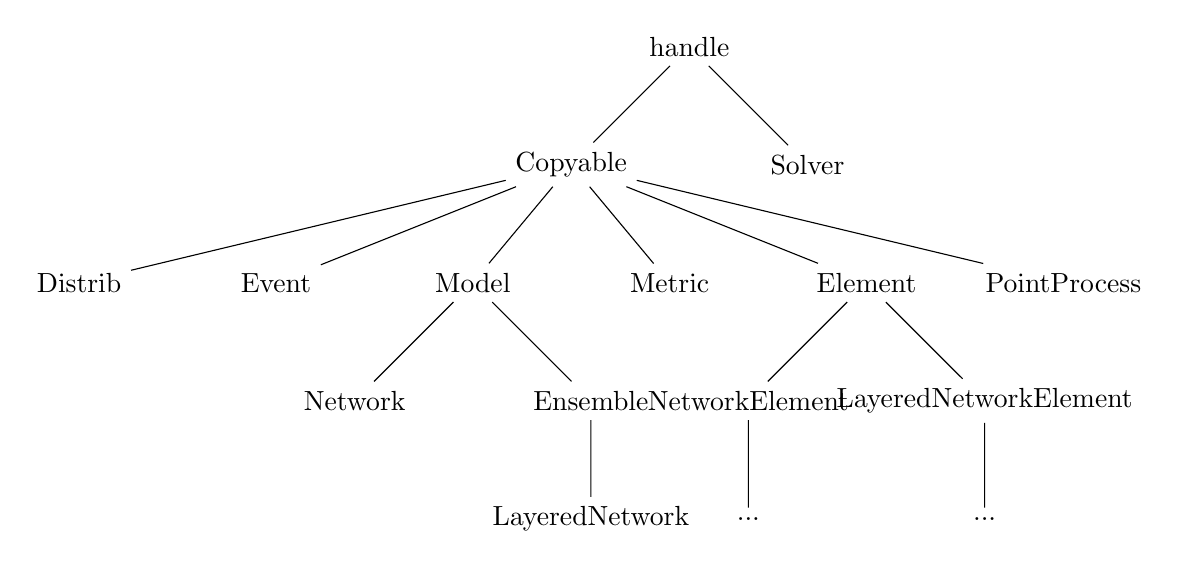
\begin{tikzpicture}[
level 1/.style={sibling distance=3.0cm},
level 2/.style={sibling distance=2.5cm},
level 3/.style={sibling distance=3.0cm},]
\node  {handle}
    child { node {Copyable}
        child { node {Distrib} }
        child { node {Event} }
        child { node {Model}
            child { node {Network} }
            child { node {Ensemble}
                  child { node {LayeredNetwork} }
            }
        }
        child { node {Metric} }
        child { node {Element}
            child { node {NetworkElement}
            child { node {...} }
            }
            child { node {LayeredNetworkElement}
            child { node {...} }
            }
        }
        child { node {PointProcess} }
    }
        child { node {Solver} } 	;
 \end{tikzpicture}
}
\end{center}
The classes in the diagram are as follows:
\begin{itemize}
\item \texttt{Copyable} allows one to perform deep-copy of objects via the \texttt{copy()} method. The class is needed to ensure reproducible behavior in both MATLAB and Octave.
\item \texttt{Distrib} is an abstract class for statistical distributions.
\item \texttt{Element} is the parent class for all the elements that define a model, such as stations, classes, jobs, etc.
\item \texttt{Ensemble} is a class of models defined by a collection of sub-models.
\item \texttt{Event} is a class to describe a generic event occurring in a model, such as an arrival or a departure of a job. This class is used in particular in the \texttt{CTMC} and \texttt{SSA} solvers.
\item \texttt{LayeredNetwork} defines a layered queueing network model.
\item \texttt{Metric} defines an output metric, such as a performance index.
\item \texttt{Reward} is a static class providing reward function templates for CTMC analysis.
\item \texttt{Model} is the parent class for all \textsc{Line} models.
\item \texttt{Network} defines an extended queueing network model.
\item \texttt{NetworkElement} defines an element in a \texttt{Network} model. The sub-hierarchy is detailed in Section~\ref{networkelement-class}.
\item \texttt{LayeredNetworkElement} defines a generic element of a \texttt{LayeredNetwork} model. The sub-hierarchy is expanded in Section~\ref{layerednetworkelement-class}.
\item \texttt{PointProcess} is an abstract class for stochastic point processes (e.g., arrival processes, service processes).
\item \texttt{Solver} is an abstract class for model solution algorithms and tools.
\end{itemize}

\section{NetworkElement class}
\label{networkelement-class}
\begin{center}
{\tiny
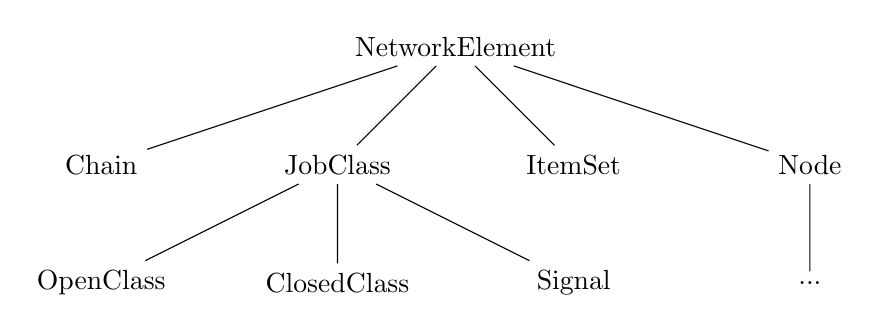
\begin{tikzpicture}[
level 1/.style={sibling distance=3cm},
level 2/.style={sibling distance=3.0cm},
level 3/.style={sibling distance=3.0cm}]
\node {NetworkElement}
                child { node {Chain}}
                child { node {JobClass}
                    child {node {OpenClass}}
                    child {node {ClosedClass}}
                    child {node {Signal}}}
                child { node {ItemSet}}
                child { node {Node}
                    child { node {...} }}
    ;
 \end{tikzpicture}
}
\end{center}
The classes in the diagram are as follows:
\begin{itemize}
\item \texttt{Chain} describes a routing chain, i.e., a collection of classes in which the job can switch its current class.
\item \texttt{JobClass} is an abstract class to describe the class of a job.
\item \texttt{OpenClass} is a class to specify an open class of jobs that arrive from a \texttt{Source} object.
\item \texttt{ClosedClass} allows one to specify a closed class of jobs that perpetually cycle within a system.
\item \texttt{Signal} extends \texttt{JobClass} and represents a signal class for G-network negative customers.
\item \texttt{ItemSet} is a class used to specify a set of cacheable items.
\item \texttt{Node} is an abstract class to describe a resource that can be visited within a network.
\item \texttt{FiniteCapacityRegion} represents a finite capacity constraint over a group of stations.
\end{itemize}

\section{LayeredNetworkElement class}
\label{layerednetworkelement-class}
\begin{center}
{\tiny
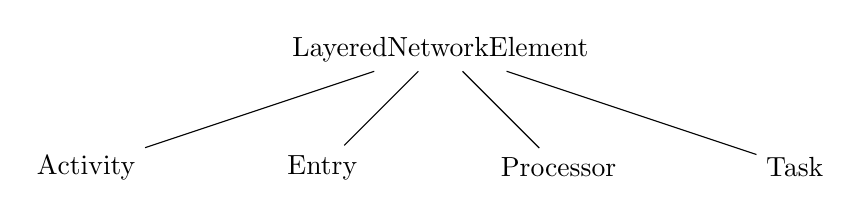
\begin{tikzpicture}[
level 1/.style={sibling distance=3.0cm},
level 2/.style={sibling distance=3.0cm},
level 3/.style={sibling distance=3.0cm},]
\node {LayeredNetworkElement}
                child { node {Activity} }
                child { node {Entry} }
                child { node {Processor} }
                child { node {Task} }
    ;
 	
 \end{tikzpicture}
}
\end{center}
The classes in the diagram are as follows:
\begin{itemize}
\item \texttt{LayeredNetworkElement} abstract class defining a generic element of a \texttt{LayeredNetwork} model.
\item \texttt{Activity} defines a stage of service in a \texttt{Task} of a \texttt{LayeredNetwork}.
\item \texttt{Entry} is a class defining an entry point for service in a \texttt{LayeredNetwork} station.
\item \texttt{Processor} defines a hardware station in a \texttt{LayeredNetwork} model.
\item \texttt{Task} defines a software station in a \texttt{LayeredNetwork} model.
\end{itemize}

\section{Node class}
\begin{center}
{\tiny
\begin{tikzpicture}[sibling distance=7.5em]
\node {NetworkElement}
    child { node {Node}
            child {node {ClassSwitch}}
            child {node {Fork}}
            child {node {Logger}}
            child {node {Router}}
            child {node {Sink}}
            child {node {StatefulNode}
                child {node {...}}
                    }
    };
 	
 \end{tikzpicture}
}
\end{center}
The classes in the diagram are as follows:
\begin{itemize}
\item \texttt{Node} is an abstract class to describe a resource that can be visited within a network.
\item \texttt{ClassSwitch} instantiates a node where jobs switch classes.
\item \texttt{Fork} instantiates a node where jobs are forked into tasks.
\item \texttt{Logger} instantiates a node where jobs are logged upon passage.
\item \texttt{Router} instantiates a node where jobs are routed to other nodes.
\item \texttt{Sink} instantiates a node where jobs in open classes depart the model.
\item \texttt{StatefulNode} is an abstract class describing a node which associated state variables.
\end{itemize}

\section{StatefulNode class}
\begin{center}
{\tiny
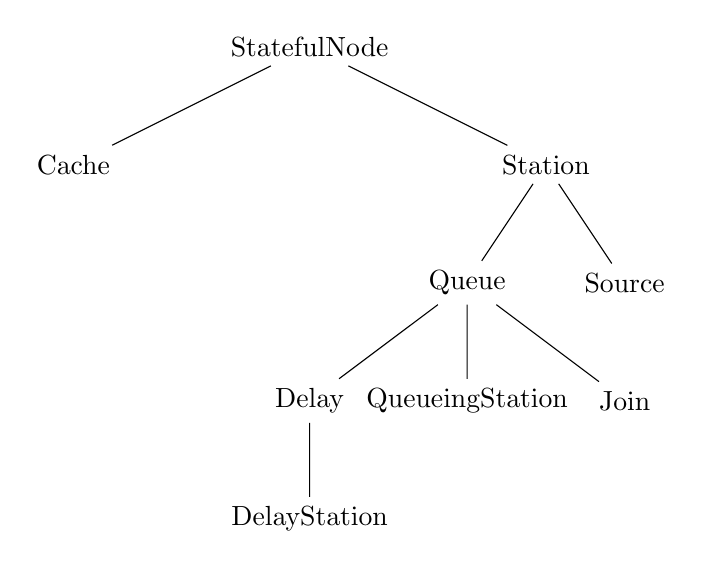
\begin{tikzpicture}[
level 1/.style={sibling distance=6cm},
level 2/.style={sibling distance=2.0cm},
level 3/.style={sibling distance=2.0cm},
level 4/.style={sibling distance=2.0cm},
level 5/.style={sibling distance=2.0cm},]
\node {StatefulNode}
                child {node {Cache}}
                child {node {Station}
                    child {node {Queue}
                        child {node {Delay}
                            child {node {DelayStation}}
                        }
                        child {node {QueueingStation}}
                        child {node {Join}}
                }
                    child {node {Source}}
    };
 	
 \end{tikzpicture}
}
\end{center}
The classes in the diagram are as follows:
\begin{itemize}
\item \texttt{StatefulNode} is an abstract class describing a node which associated state variables.
\item \texttt{Cache} instantiates a cache node.
\item \texttt{Station} is an abstract class for nodes where jobs spend time.
\item \texttt{Join} instantiates a join station.
\item \texttt{Queue} instantiates a queueing station.
\item \texttt{Delay} instantiates a delay station.
\item \texttt{DelayStation} alias for \texttt{Delay}.
\item \texttt{QueueingStation} alias for \texttt{Queue}.
\item \texttt{Source} instantiates a source from which jobs can arrive in open classes.
\item \texttt{ServerType} defines heterogeneous server types within a Queue, enabling different servers with distinct service rates and job class compatibilities.
\end{itemize}

\section{Distrib class}
\begin{center}
{\tiny
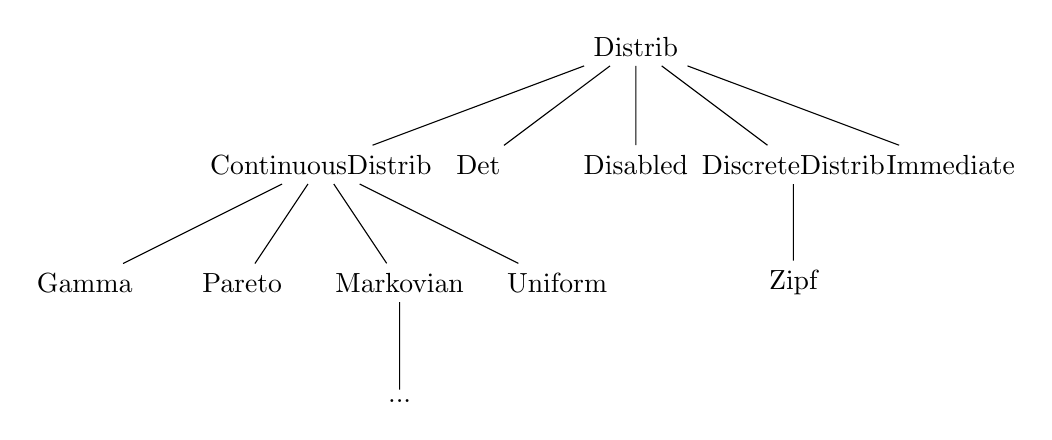
\begin{tikzpicture}[
level 1/.style={sibling distance=2cm},
level 2/.style={sibling distance=2cm},
level 3/.style={sibling distance=2.0cm},
level 4/.style={sibling distance=2.0cm},
level 5/.style={sibling distance=2.0cm},]
\node {Distrib}
            child {node {ContinuousDistrib}
                child {node {Gamma}}
                child {node {Pareto}}
                child {node {Markovian}
                    child {node {...}}
                }
                child {node {Uniform}}
            }
            child {node {Det}}
            child {node {Disabled}}
            child {node {DiscreteDistrib}
                child {node {Zipf}}
            }
            child {node {Immediate}}
            ;
 	
 \end{tikzpicture}
}
\end{center}
The classes in the diagram are as follows:
\begin{itemize}
\item \texttt{Distrib} is an abstract class for statistical distributions.
\item \texttt{ContinuousDistrib} is an abstract class for distributions defined over a continuous interval.
\item \texttt{Det} instantiates a deterministic distribution.
\item \texttt{Disabled} is a placeholder class for a distribution that is disabled or unspecified.
\item \texttt{DiscreteDistrib} is an abstract class for distributions defined at discrete point.
\item \texttt{Zipf} defines a Zipf distribution.
\item \texttt{Immediate} defines a deterministic distribution with mass entirely at 0.
\item \texttt{Pareto} defines a Pareto distribution.
\item \texttt{Markovian} is an abstract class for phase-type distributions.
\item \texttt{Uniform} defines a uniform distribution over a bounded range.
\item \texttt{Prior} extends \texttt{Distribution} and represents a prior distribution for Bayesian parameter uncertainty.
\end{itemize}

\section{Markovian class}
\begin{center}
{\tiny
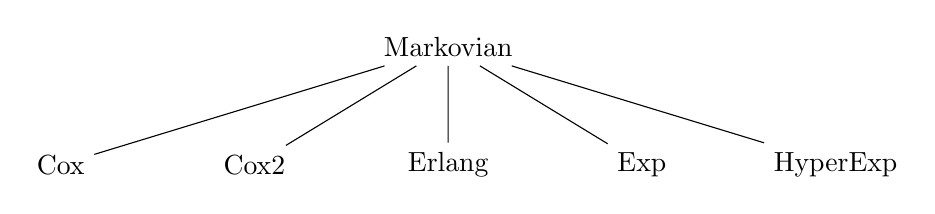
\begin{tikzpicture}[sibling distance=7em]
\node {Markovian}
        child {node {Cox}}
        child {node {Cox2}}
        child {node {Erlang}}
        child {node {Exp}}
        child {node {HyperExp}}
             ; 	
 \end{tikzpicture}
}
\end{center}
The classes in the diagram are as follows:
\begin{itemize}
\item \texttt{Markovian} is an abstract class for phase-type distributions.
\item \texttt{Cox} is a class for Coxian distributions with arbitrary number of phases.
\item \texttt{Cox2} is a class for 2-phase Coxian distributions.
\item \texttt{Erlang} is a class for Erlang distributions with arbitrary number of phases.
\item \texttt{Exp} instantiates an exponential distribution.
\item \texttt{HyperExp} is a class for 2-phase hyper-exponential distributions.
\end{itemize}

\section{PointProcess class}
\begin{center}
{\tiny
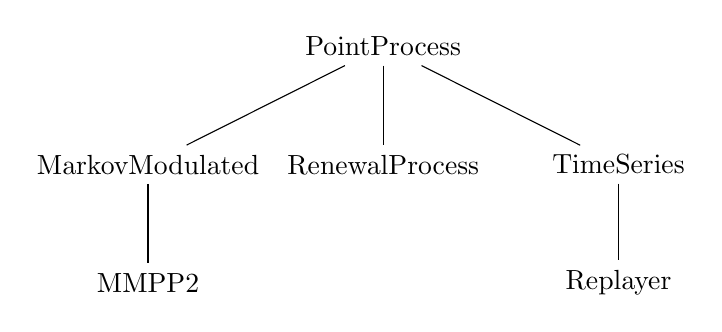
\begin{tikzpicture}[sibling distance=8.5em]
\node {PointProcess}
            child {node {MarkovModulated}
                child {node {MMPP2}}
                }
            child {node {RenewalProcess}}
            child {node {TimeSeries}
                child {node {Replayer}}
                }
             ;
 	
 \end{tikzpicture}
}
\end{center}
The classes in the diagram are as follows:
\begin{itemize}
\item \texttt{PointProcess} is an abstract class for stochastic point processes (e.g., arrival processes, service processes).
\item \texttt{MarkovModulated} is an abstract class for Markov-modulated point processes.
\item \texttt{MMPP2} instantiates a Markov-Modulation Poisson Process with 2-states.
\item \texttt{RenewalProcess} is a class to instantiate processes with i.i.d. samples from an object that inherits from \texttt{Distrib}
\item \texttt{TimeSeries} is an abstract class for empirical point processes.
\item \texttt{Replayer} is a class that loads a time series from a file. \texttt{Trace} is an alias for \texttt{Replayer}.
\end{itemize}

\section{Section class}
\begin{center}
{\tiny
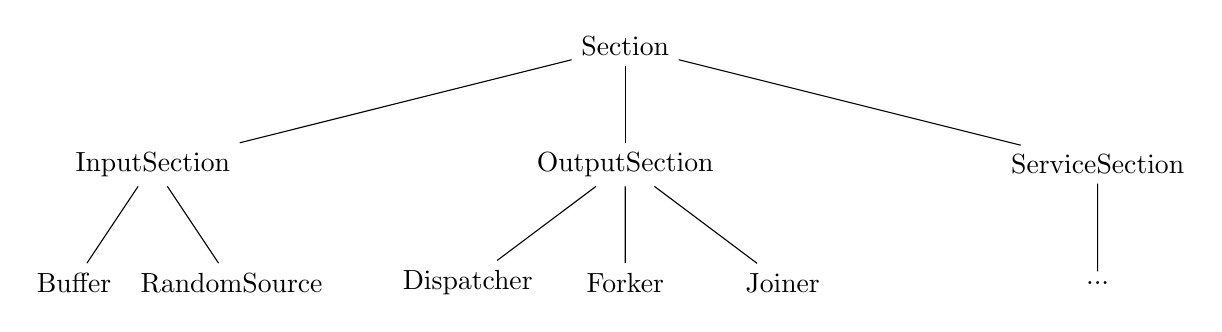
\begin{tikzpicture}[
level 1/.style={sibling distance=6cm},
level 2/.style={sibling distance=2.0cm},
level 3/.style={sibling distance=2.0cm},
level 4/.style={sibling distance=2.0cm},
level 5/.style={sibling distance=2.0cm},]
\node  {Section}
                child {node {InputSection}
                    child {node {Buffer}}
                    child {node {RandomSource}}}
                child {node {OutputSection}
                    child {node {Dispatcher}}
                    child {node {Forker}}
                    child {node {Joiner}}}
                child {node {ServiceSection}
                    child {node {...}}}
             ;
 	
 \end{tikzpicture}
}
\end{center}
The classes in the diagram are as follows:
\begin{itemize}
\item \texttt{Section} is an abstract class defining a section part of a node.
\item \texttt{InputSection} is an abstract class for sections defining the handling of jobs waiting to be served.
\item \texttt{Buffer} is a class defining a waiting buffer.
\item \texttt{RandomSource} is a class defining the generation of jobs in open classes.
\item \texttt{OutputSection} is an abstract class for sections defining the node behaviour after completing service.
\item \texttt{Dispatcher} is a class implementing routing towards another node.
\item \texttt{Forker} is a section forking a job into a set of sibling tasks.
\item \texttt{Joiner} is a section merging sibling tasks into the original job.
\item \texttt{ServiceSection} is an abstract class for sections defining the node behaviour during service.
\end{itemize}

\section{ServiceSection class}
\begin{center}
{\tiny
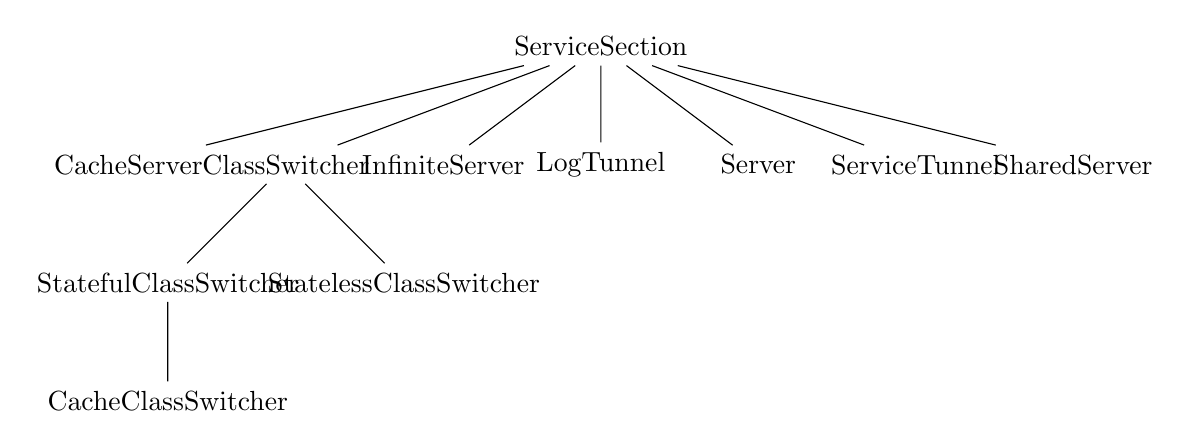
\begin{tikzpicture}[
level 1/.style={sibling distance=2cm},
level 2/.style={sibling distance=3.0cm},
level 3/.style={sibling distance=2.5cm},
level 4/.style={sibling distance=2.5cm},
level 5/.style={sibling distance=2.0cm},]
\node {ServiceSection}
            child {node {CacheServer}}
            child {node {ClassSwitcher}
                child {node {StatefulClassSwitcher}
                   child {node {CacheClassSwitcher}}
                }
                child {node {StatelessClassSwitcher}}
            }
            child {node {InfiniteServer}}
            child {node {LogTunnel}}
            child {node {Server}}
            child {node {ServiceTunnel}}
            child {node {SharedServer}}
            ;
 	
 \end{tikzpicture}
}
\end{center}
The classes in the diagram are as follows:
\begin{itemize}
\item \texttt{ServiceSection} is an abstract class for sections defining the node behaviour during service.
\item \texttt{CacheServer} is a section tracking and updating the cache state.
\item \texttt{ClassSwitcher} is an abstract class for sections changing the class of a visiting job or task.
\item \texttt{StatefulClassSwitcher} is an abstract class for \texttt{ClassSwitcher} sections that depend on the node state.
\item \texttt{CacheClassSwitcher} is a \texttt{StatefulClassSwitcher} that depends on the cache state.
\item \texttt{StatelessClassSwitcher} is an abstract class for \texttt{ClassSwitcher} sections that depend on a static rule.
\item \texttt{InfiniteServer} is a section for non-preemptive service with an infinite level of parallelism.
\item \texttt{LogTunnel} is a dummy service section for \texttt{Logger} nodes.
\item \texttt{Server} is a section for non-preemptive service with a finite level of parallelism. This section includes serial service as a special case.
\item \texttt{ServiceTunnel} is a dummy service section for nodes that do not serve jobs.
\item \texttt{SharedServer} is a section for preemptive service (e.g., processor sharing)
\end{itemize}

\section{Solver class}
\begin{center}
{\tiny
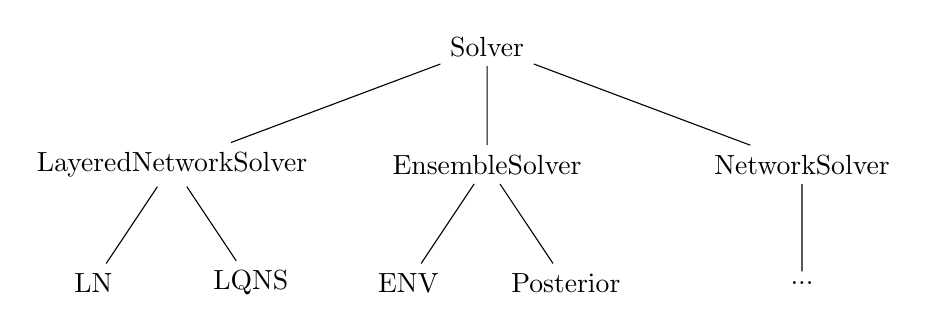
\begin{tikzpicture}[
level 1/.style={sibling distance=4cm},
level 2/.style={sibling distance=2.0cm},
level 3/.style={sibling distance=2.0cm},
level 4/.style={sibling distance=2.5cm},
level 5/.style={sibling distance=2.0cm},]
\node  {Solver}
        child { node {LayeredNetworkSolver}
            child { node {LN} }
            child { node {LQNS} }
        }
        child { node {EnsembleSolver}
            child { node {ENV} }
            child { node {Posterior} }
        }
        child { node {NetworkSolver}
            child { node {...} }
        }
    ;
 	
 \end{tikzpicture}
}
\end{center}
The classes in the diagram are as follows:
\begin{itemize}
\item \texttt{Solver} is an abstract class for model solution algorithms and tools.
\item \texttt{LayeredNetworkSolver} is an abstract class for solvers of \texttt{LayeredNetwork} models.
\item \texttt{LN} implements the \texttt{LN} layered queueing network solver.
\item \texttt{LQNS} implements the interface to the \texttt{LQNS} layered queueing network solver.
\item \texttt{EnsembleSolver}  is an abstract class for solvers of models with random environments.
\item \texttt{ENV} implements the \texttt{Env} random environment solver.
\item \texttt{Posterior} extends \texttt{EnsembleSolver} and is a meta-solver for models with Prior distributions.
\item \texttt{NetworkSolver} is an abstract class for solvers of \texttt{Network} models.
\end{itemize}

\section{NetworkSolver class}
\begin{center}
{\tiny
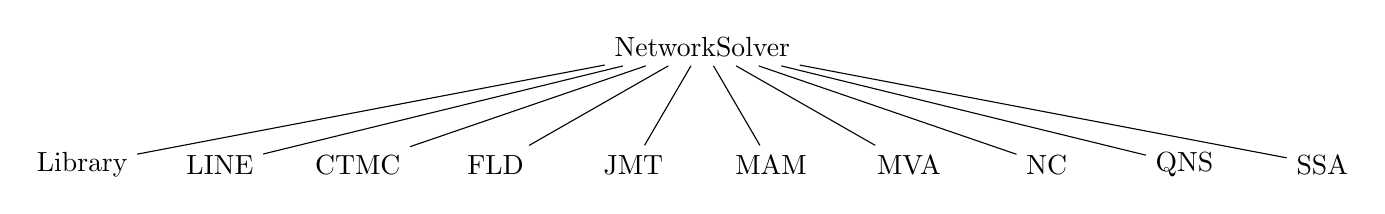
\begin{tikzpicture}[
level 1/.style={sibling distance=1.75cm},
level 2/.style={sibling distance=2.0cm},
level 3/.style={sibling distance=2.0cm},
level 4/.style={sibling distance=2.5cm},
level 5/.style={sibling distance=2.0cm},]
\node  {NetworkSolver}
            child { node {Library} }
            child { node {LINE} }
            child { node {CTMC} }
            child { node {FLD} }
            child { node {JMT} }
            child { node {MAM} }
            child { node {MVA} }
            child { node {NC} }
            child { node {QNS} }
            child { node {SSA} }

    ;
 	
 \end{tikzpicture}
}
\end{center}
The classes in the diagram are as follows:
\begin{itemize}
\item \texttt{NetworkSolver} is the abstract class defining a generic solver for extended queueing network.
\item \texttt{Library} collection of ad-hoc solution methods for extended queueing networks.
\item \texttt{LINE} instantiates a meta-solver that recommends the solver to run for a given model.
\item \texttt{CTMC} instantiates the \texttt{CTMC} solver.
\item \texttt{JMT} instantiates the \texttt{JMT} solver.
\item \texttt{MAM} instantiates the \texttt{MAM} solver.
\item \texttt{MVA} instantiates the \texttt{MVA} solver.
\item \texttt{NC} instantiates the \texttt{NC} solver.
\item \texttt{QNS} instantiates \texttt{LQNS}'s qnsolver.
\item \texttt{SSA} instantiates the \texttt{SSA} solver.
\end{itemize}    
\end{comment}

\chapter{API Function Reference}
\label{ch:api-function-reference}

This appendix provides a comprehensive catalog of all API functions available in the \texttt{jline.api} package. The table lists each function name, its organizational package, and a brief description of its purpose.

\begin{footnotesize}
\begin{longtable}{|p{0.4\linewidth}|p{0.1\linewidth}|p{0.5\linewidth}|}
\caption{Complete API Function Reference}
\label{tab:api-functions}
\\\hline
\textbf{Function Name} & \textbf{Package} & \textbf{Description}
\\\hline
\endfirsthead
\multicolumn{3}{c}%
{\tablename\ \thetable\ -- API Function Reference.\textit{ Continued from previous page}} \\
\hline
\textbf{Function Name} & \textbf{Package} & \textbf{Description}\\
\hline
\endhead
\hline \multicolumn{3}{r}{\textit{Continued on next page}} \\
\endfoot
\hline
\endlastfoot
\texttt{amap2\_fit\_gamma} & mam & Fits AMAP(2) distributions to match moments and correlation characteristics\\
\texttt{amap2\_fit\_gamma\_map} & mam & Fits AMAP(2) by approximating arbitrary-order MAP with preserved correlation structure\\
\texttt{amap2\_fit\_gamma\_trace} & mam & Fits AMAP(2) from empirical traces while preserving autocorrelation characteristics\\
\texttt{aph2\_adjust} & mam & Adjusts moments to ensure feasibility bounds for APH(2) fitting procedures\\
\texttt{aph2\_assemble} & mam & Constructs APH(2) transition matrices from specified rates and transition probabilities\\
\texttt{aph2\_fit} & mam & Fits APH(2) distributions to match given moments with automatic feasibility adjustment\\
\texttt{aph2\_fit\_map} & mam & Fits APH(2) distributions by approximating arbitrary-order MAP processes\\
\texttt{aph2\_fit\_trace} & mam & Fits APH(2) distributions from empirical inter-arrival time traces\\
\texttt{aph2\_fitall} & mam & Fits multiple APH(2) distributions to match given moments with exhaustive parameter search\\
\texttt{aph\_bernstein} & mam & Constructs APH distributions using Bernstein exponential approximation methods\\
\texttt{aph\_fit} & mam & Fits APH distributions to specified moments using optimization and approximation techniques\\
\texttt{aph\_rand} & mam & APH random generation algorithms\\
\texttt{aph\_simplify} & mam & Simplifies and combines APH distributions using structural pattern operations\\
\texttt{cache\_erec} & cache & Implements exact recursive (EREC) algorithms for cache system analysis\\
\texttt{cache\_gamma} & cache & Computes cache access factors from request arrival rates and routing matrices\\
\texttt{cache\_gamma\_lp} & cache & Computes cache access factors using linear programming optimization methods\\
\texttt{cache\_miss} & cache & Provides general-purpose algorithms for computing cache miss rates across\\
\texttt{cache\_miss\_asy} & cache & Provides asymptotic approximation methods for cache miss rate analysis\\
\texttt{cache\_miss\_fpi} & cache & Computes cache miss probabilities using fixed-point iteration methods\\
\texttt{cache\_miss\_rayint} & cache & Estimates cache miss rates using ray method for partial differential equations\\
\texttt{cache\_mva} & cache & Implements Mean Value Analysis algorithms for cache system performance\\
\texttt{cache\_mva\_miss} & cache & Implements Mean Value Analysis (MVA) algorithms for computing cache miss\\
\texttt{cache\_prob\_erec} & cache & Computes exact cache state probabilities using recursive methods based on\\
\texttt{cache\_prob\_fpi} & cache & Computes cache state probabilities using fixed-point iteration algorithms\\
\texttt{cache\_prob\_rayint} & cache & Computes cache state probabilities using ray integration methods for\\
\texttt{cache\_rayint} & cache & Implements ray integration techniques for cache system analysis using\\
\texttt{cache\_rrm\_meanfield\_ode} & cache & Implements the mean field ordinary differential equation system for Random\\
\texttt{cache\_t\_hlru} & cache & Computes response time metrics for Hierarchical Least Recently Used (H-LRU)\\
\texttt{cache\_t\_lrum} & cache & Computes response time metrics for Least Recently Used with Multiple servers\\
\texttt{cache\_t\_lrum\_map} & cache & Analyzes response times for LRUM cache systems with Markovian Arrival\\
\texttt{cache\_ttl\_hlru} & cache & Implements TTL approximation for Hierarchical LRU (H-LRU) cache systems\\
\texttt{cache\_ttl\_lrua} & cache & Implementation of Time-To-Live (TTL) approximation for LRU(A) cache systems\\
\texttt{cache\_ttl\_lrum} & cache & Implementation of Time-To-Live approximation for Least Recently Used with\\
\texttt{cache\_ttl\_lrum\_map} & cache & Combines TTL approximation with LRUM cache policies and Markovian Arrival\\
\texttt{cache\_ttl\_tree} & cache & Tree-based TTL cache analysis implementation for the LINE solver framework\\
\texttt{cache\_xi\_bvh} & cache & Computes cache xi terms using the iterative method from Gast-van Houdt\\
\texttt{cache\_xi\_fp} & cache & Estimates cache xi terms using fixed-point algorithms. Xi terms represent\\
\texttt{ctmc\_courtois} & mc & Courtois decomposition for nearly completely decomposable CTMCs\\
\texttt{ctmc\_kms} & mc & Koury-McAllister-Stewart aggregation-disaggregation method for CTMCs\\
\texttt{ctmc\_makeinfgen} & mc & Constructs and validates infinitesimal generator matrices for continuous-time\\
\texttt{ctmc\_multi} & mc & Multi-level aggregation method for CTMCs\\
\texttt{ctmc\_pseudostochcomp} & mc & API function for mc operations\\
\texttt{ctmc\_rand} & mc & Generates random infinitesimal generator matrices for continuous-time Markov chains\\
\texttt{ctmc\_randomization} & mc & Converts a continuous-time Markov chain into an equivalent discrete-time chain\\
\texttt{ctmc\_relsolve} & mc & Equilibrium distribution of a continuous-time Markov chain re-normalized with respect to\\
\texttt{ctmc\_simulate} & mc & Generates sample paths for CTMCs using the standard simulation algorithm with\\
\texttt{ctmc\_solve} & mc & Computes the steady-state probability distribution for CTMCs by solving the linear\\
\texttt{ctmc\_solve\_reducible} & mc & Solve reducible CTMCs by converting to DTMC via randomization\\
\texttt{ctmc\_ssg} & mc & API function for mc operations\\
\texttt{ctmc\_ssg\_reachability} & mc & CTMC State Space Generator for Reachability Analysis\\
\texttt{ctmc\_stmonotone} & mc & Computes the stochastically monotone upper bound for a CTMC\\
\texttt{ctmc\_stochcomp} & mc & Implements stochastic complementarity analysis for CTMCs to identify strongly\\
\texttt{ctmc\_takahashi} & mc & Takahashi's aggregation-disaggregation method for CTMCs\\
\texttt{ctmc\_testpf\_kolmogorov} & mc & Test if a CTMC has product form using Kolmogorov's criteria\\
\texttt{ctmc\_timereverse} & mc & Computes the infinitesimal generator of the time-reversed continuous-time\\
\texttt{ctmc\_transient} & mc & Computes transient probabilities for CTMCs using numerical integration of the\\
\texttt{ctmc\_uniformization} & mc & CTMC Transient Analysis via Uniformization\\
\texttt{dtmc\_isfeasible} & mc & Check if a matrix represents a feasible DTMC transition matrix\\
\texttt{dtmc\_makestochastic} & mc & Converts non-negative matrices into valid discrete-time Markov chain transition\\
\texttt{dtmc\_rand} & mc & Generates random stochastic transition matrices for discrete-time Markov chains\\
\texttt{dtmc\_simulate} & mc & Generates sample trajectories for DTMCs by sampling from the transition probability\\
\texttt{dtmc\_solve} & mc & Computes the steady-state probability distribution for DTMCs by converting the\\
\texttt{dtmc\_solve\_reducible} & mc & Result class for DTMC solve reducible\\
\texttt{dtmc\_stochcomp} & mc & Returns the stochastic complement of a DTMC\\
\texttt{dtmc\_timereverse} & mc & Compute the infinitesimal generator of the time-reversed DTMC\\
\texttt{dtmc\_uniformization} & mc & Result class for DTMC uniformization analysis containing the probability vector and maximum iterations used\\
\texttt{lossn\_erlangfp} & lossn & Implements fixed-point algorithms for analyzing loss networks using Erlang\\
\texttt{lsn\_max\_multiplicity} & lsn & Computes maximum multiplicity constraints for load sharing network (LSN)\\
\texttt{m3pp22\_fitc\_approx\_cov} & mam.m3pp & Implements parameter fitting for second-order Marked Markov Modulated Poisson Process\\
\texttt{m3pp22\_fitc\_approx\_cov\_multiclass} & mam.m3pp & Implements constrained optimization for fitting M3PP(2,2) parameters given an underlying\\
\texttt{m3pp22\_interleave\_fitc} & mam.m3pp & Implements lumped superposition of multiple M3PP(2,2) processes using interleaved\\
\texttt{m3pp2m\_fitc} & mam.m3pp & Implements exact fitting of second-order Marked Markov Modulated Poisson Process\\
\texttt{m3pp2m\_fitc\_approx} & mam.m3pp & Implements approximation-based fitting for M3PP(2,m) using optimization methods\\
\texttt{m3pp2m\_fitc\_approx\_ag} & mam.m3pp & Implements auto-gamma approximation method for M3PP(2,m) parameter fitting\\
\texttt{m3pp2m\_fitc\_approx\_ag\_multiclass} & mam.m3pp & Implements multiclass auto-gamma fitting for M3PP(2,m) with variance and covariance\\
\texttt{m3pp2m\_interleave} & mam.m3pp & Implements interleaved superposition of multiple M3PP(2,m) processes to construct\\
\texttt{m3pp\_interleave\_fitc} & mam.m3pp & Implements fitting and interleaving of k second-order M3PP processes with varying\\
\texttt{m3pp\_interleave\_fitc\_theoretical} & mam.m3pp & Implements theoretical MMAP fitting through M3PP interleaving using analytical\\
\texttt{m3pp\_interleave\_fitc\_trace} & mam.m3pp & Implements M3PP interleaving and fitting directly from empirical trace data\\
\texttt{m3pp\_rand} & mam.m3pp & Implements random generation of Markovian Multi-class Point Processes (M3PP)\\
\texttt{m3pp\_superpos\_fitc} & mam.m3pp & Implements superposition-based fitting of k second-order M3PP processes into\\
\texttt{m3pp\_superpos\_fitc\_theoretical} & mam.m3pp & Implements superposition fitting of k second-order M3PP processes using theoretical\\
\texttt{mamap22\_fit\_gamma\_fs\_trace} & mam & Fits MAMAP(2,2) from trace data using gamma autocorrelation and forward-sigma characteristics\\
\texttt{mamap22\_fit\_multiclass} & mam & Fits MAMAP(2,2) processes for two-class systems with forward moments and sigma characteristics\\
\texttt{mamap2m\_coefficients} & mam & Computes coefficients for MAMAP(2,m) fitting formulas in canonical forms\\
\texttt{mamap2m\_fit} & mam & Fits MAMAP(2,m) processes matching moments, autocorrelation, and class characteristics\\
\texttt{mamap2m\_fit\_fb\_multiclass} & mam & Fits MAMAP using combined forward and backward moment characteristics for multiclass systems\\
\texttt{mamap2m\_fit\_gamma\_fb\_mmap} & mam & Fits MAMAP with autocorrelation control using forward-backward moments from MMAP input\\
\texttt{mamap2m\_fit\_mmap} & mam & Fits MAPH/MAMAP(2,m) by approximating characteristics of input MMAP processes\\
\texttt{mamap2m\_fit\_trace} & mam & Fits MAMAP(2,m) processes from empirical trace data with inter-arrival times and class labels\\
\texttt{map2\_fit} & mam & Fits MAP(2) processes to match specified moments and autocorrelation decay rates\\
\texttt{map2mmpp} & mam & Converts MAP representations to MMPP format for compatibility with MMPP-specific algorithms\\
\texttt{map\_acf} & mam & Computes autocorrelation function (ACF) values for MAP inter-arrival times at specified lags\\
\texttt{map\_acfc} & mam & Computes ACFC values for MAP counting processes over time intervals, measuring temporal correlation\\
\texttt{map\_block} & mam & Constructs MAP(2) representations from moment and autocorrelation parameters using fallback\\
\texttt{map\_ccdf\_derivative} & mam & Computes derivatives of MAP complementary cumulative distribution functions at zero\\
\texttt{map\_cdf} & mam & Computes CDF values for MAP inter-arrival times using CTMC uniformization techniques\\
\texttt{map\_checkfeasible} & mam & Comprehensive validation of MAP matrices including stochastic properties, numerical stability,\\
\texttt{map\_count\_mean} & mam & Computes mean number of arrivals in MAP counting processes over specified time intervals\\
\texttt{map\_count\_moment} & mam & Computes power moments of MAP counting processes using moment generating functions and\\
\texttt{map\_count\_var} & mam & Computes variance of MAP counting processes over specified time intervals using matrix\\
\texttt{map\_embedded} & mam & Computes embedded DTMC matrices from MAP representations by extracting transition\\
\texttt{map\_erlang} & mam & Constructs MAP representations of Erlang-k processes with specified means and phases\\
\texttt{map\_exponential} & mam & Creates MAP representations of exponential inter-arrival time distributions with specified\\
\texttt{map\_feasblock} & mam & Constructs feasible MAP representations when exact moment matching fails by adjusting\\
\texttt{map\_feastol} & mam & Provides standard tolerance values for numerical feasibility checks in MAP algorithms\\
\texttt{map\_gamma} & mam & Computes gamma parameter measuring autocorrelation decay rates in MAP processes\\
\texttt{map\_gamma2} & mam & Computes largest non-unit eigenvalue of embedded DTMC for MAP correlation characterization\\
\texttt{map\_hyperexp} & mam & Constructs MAP representations of two-phase hyperexponential renewal processes\\
\texttt{map\_idc} & mam & Computes asymptotic index of dispersion for MAP counting processes, measuring long-term\\
\texttt{map\_infgen} & mam & Computes infinitesimal generator matrix of underlying CTMC by combining MAP transition\\
\texttt{map\_isfeasible} & mam & Provides convenient interface for MAP feasibility validation with configurable tolerance\\
\texttt{map\_joint} & mam & Computes joint moments of MAP inter-arrival times for advanced statistical characterization\\
\texttt{map\_jointpdf\_derivative} & mam & Computes partial derivatives of MAP joint probability density functions at origin\\
\texttt{map\_kpc} & mam & Computes Kronecker product composition of multiple MAPs for building complex arrival processes\\
\texttt{map\_kurt} & mam & Computes kurtosis of MAP inter-arrival times measuring tail heaviness and distribution shape\\
\texttt{map\_lambda} & mam & MAP arrival rate computation algorithms\\
\texttt{map\_largemap} & mam & Provides size thresholds for determining when MAP algorithms should switch to\\
\texttt{map\_mark} & mam & Creates Marked MAP (MMAP) representations by adding class labels to MAP arrivals\\
\texttt{map\_max} & mam & Computes MAP representation of maximum inter-arrival times from independent MAP processes\\
\texttt{map\_mean} & mam & MAP mean inter-arrival time computation algorithms\\
\texttt{map\_mixture} & mam & Creates probabilistic mixtures of MAP processes with specified mixture probabilities\\
\texttt{map\_moment} & mam & Computes raw moments of MAP inter-arrival times using matrix inversion techniques\\
\texttt{map\_normalize} & mam & Sanitizes MAP matrices by ensuring non-negativity constraints and proper diagonal adjustments\\
\texttt{map\_pdf} & mam & Computes PDF values for MAP inter-arrival times using matrix exponential techniques\\
\texttt{map\_pie} & mam & Computes steady-state probability vector of embedded discrete-time Markov chain\\
\texttt{map\_piq} & mam & Computes steady-state probability vector of underlying continuous-time Markov chain\\
\texttt{map\_pntiter} & mam & Computes exact arrival probabilities using iterative numerical methods based on Neuts and Li\\
\texttt{map\_pntquad} & mam & Computes MAP point process probabilities using ODE quadrature methods with Runge-Kutta integration\\
\texttt{map\_prob} & mam & Computes equilibrium probability distribution of underlying CTMC for MAP analysis\\
\texttt{map\_rand} & mam & Generates random MAP representations for testing, simulation, and statistical analysis\\
\texttt{map\_randn} & mam & Generates random MAP samples with added numerical noise for robustness testing\\
\texttt{map\_renewal} & mam & Creates renewal MAP by removing correlations to obtain memoryless arrival processes\\
\texttt{map\_sample} & mam & Generates random samples from MAP distributions for simulation and empirical analysis\\
\texttt{map\_scale} & mam & Rescales MAP inter-arrival time distributions to achieve specified mean values\\
\texttt{map\_scv} & mam & Computes SCV of MAP inter-arrival times as normalized dispersion measure\\
\texttt{map\_skew} & mam & Computes skewness of MAP inter-arrival times measuring asymmetry in distributions\\
\texttt{map\_stochcomp} & mam & Performs state elimination through stochastic complementation while preserving MAP properties\\
\texttt{map\_sum} & mam & Computes MAP representations of sums of identical MAP processes for load scaling\\
\texttt{map\_sumind} & mam & Computes MAP representations of sums of independent MAP processes for modeling\\
\texttt{map\_super} & mam & Creates superposition of MAP processes using Kronecker product techniques\\
\texttt{map\_timereverse} & mam & Computes time-reversed MAP by adjusting transition rates based on stationary distributions\\
\texttt{map\_var} & mam & MAP variance computation algorithms\\
\texttt{map\_varcount} & mam & Computes variance of event counts in MAP processes over specified time intervals\\
\texttt{maph2m\_fit} & mam & Fits MAPH(2,m) processes to match ordinary moments, class probabilities, and backward moments\\
\texttt{maph2m\_fit\_mmap} & mam & Fits MAPH(2,m) by approximating characteristics of input MMAP processes\\
\texttt{maph2m\_fit\_multiclass} & mam & Fits MAPH(2,m) models to multiclass characteristics with class-specific parameters\\
\texttt{maph2m\_fit\_trace} & mam & Fits MAPH(2,m) from empirical trace data for multiclass service time modeling\\
\texttt{maph2m\_fitc\_approx} & mam & Fits MAPH(2,m) using approximation methods for count statistics when exact solutions fail\\
\texttt{maph2m\_fitc\_theoretical} & mam & Fits MAPH(2,m) using theoretical count statistics for precise parameter estimation\\
\texttt{mapqn\_bnd\_lr} & mapqn & Implements general linear reduction methods for computing performance\\
\texttt{mapqn\_bnd\_lr\_mva} & mapqn & Implements linear reduction bounds for MAP queueing networks using Mean\\
\texttt{mapqn\_bnd\_lr\_pf} & mapqn & Implements linear reduction bounds specialized for product-form MAP\\
\texttt{mapqn\_bnd\_qr} & mapqn & Implements general quadratic reduction methods for computing performance\\
\texttt{mapqn\_bnd\_qr\_delay} & mapqn & Implements quadratic reduction bounds for delay systems in MAP queueing\\
\texttt{mapqn\_bnd\_qr\_ld} & mapqn & Implements quadratic reduction bounds for load-dependent MAP queueing\\
\texttt{mapqn\_lpmodel} & mapqn & Base class for representing MAP queueing network linear programming models\\
\texttt{mapqn\_parameters} & mapqn & Defines the base parameter structure for MAP queueing network analysis\\
\texttt{mapqn\_parameters\_factory} & mapqn & Factory class for creating parameter objects for MAP queueing network\\
\texttt{mapqn\_qr\_bounds\_bas} & mapqn & Implements Queue-Router bounds using the Balanced Asymptotic Scaling (BAS)\\
\texttt{mapqn\_qr\_bounds\_rsrd} & mapqn & Implements Queue-Router (QR) bounds using the Randomized Simultaneous\\
\texttt{mmap\_backward\_moment} & mam & Computes backward moments of MMAP inter-arrival times for each marked class\\
\texttt{mmap\_compress} & mam & Compresses MMAP using various approximation methods including mixture, matching,\\
\texttt{mmap\_count\_idc} & mam & Computes IDC values for each marked class in MMAP counting processes\\
\texttt{mmap\_count\_lambda} & mam & Computes arrival rate vectors for each marked class in MMAP processes\\
\texttt{mmap\_count\_mcov} & mam & Computes count covariance matrices between marked classes in MMAP processes\\
\texttt{mmap\_count\_mean} & mam & Computes mean count vectors for each marked class in MMAP counting processes\\
\texttt{mmap\_count\_var} & mam & Computes variance vectors for counting processes of each marked class in MMAP\\
\texttt{mmap\_cross\_moment} & mam & Computes cross-moment matrices between different marked classes in MMAP processes\\
\texttt{mmap\_embedded} & mam & Computes embedded discrete-time Markov chain for MMAP processes\\
\texttt{mmap\_exponential} & mam & Constructs MMAP with exponential inter-arrival distributions for each marked class\\
\texttt{mmap\_forward\_moment} & mam & Computes forward moments of MMAP inter-arrival times for each marked class\\
\texttt{mmap\_hide} & mam & Hides specified arrival classes in MMAP processes by removing observable events\\
\texttt{mmap\_idc} & mam & Computes asymptotic IDC for each marked class in MMAP as time approaches infinity\\
\texttt{mmap\_isfeasible} & mam & Validates mathematical feasibility of MMAP representations including stochastic\\
\texttt{mmap\_issym} & mam & Checks if an MMAP is symmetric\\
\texttt{mmap\_lambda} & mam & MMAP arrival rate computation algorithms\\
\texttt{mmap\_maps} & mam & Extracts individual MAP processes for each marked class from MMAP representations\\
\texttt{mmap\_mark} & mam & Converts a Markovian Arrival Process with marked arrivals (MMAP) into a new MMAP with redefined classes based on a given probability matrix\\
\texttt{mmap\_max} & mam & Computes element-wise maximum of MMAP processes for synchronization analysis\\
\texttt{mmap\_mixture} & mam & Creates probabilistic mixtures of MMAP processes with specified weights\\
\texttt{mmap\_mixture\_fit} & mam & Fits a mixture of Markovian Arrival Processes (MMAPs) to match the given cross-moments\\
\texttt{mmap\_mixture\_fit\_mmap} & mam & Fits a mixture of Markovian Arrival Processes (MMAPs) to match the given moments\\
\texttt{mmap\_mixture\_order2} & mam & Creates a second-order MMAP mixture from a collection of MMAPs\\
\texttt{mmap\_modulate} & mam & Modulates an MMAP by another MMAP, creating a compound arrival process\\
\texttt{mmap\_normalize} & mam & Normalizes MMAP matrices to ensure feasibility and mathematical validity\\
\texttt{mmap\_pc} & mam & Computes the proportion of counts (PC) for each type in a Markovian Arrival Process with marked arrivals (MMAP)\\
\texttt{mmap\_pie} & mam & Computes steady-state probability vectors for each marked class in MMAP processes\\
\texttt{mmap\_rand} & mam & Generates random MMAP representations for testing and simulation purposes\\
\texttt{mmap\_sample} & mam & Generates random samples from MMAP distributions for each marked class\\
\texttt{mmap\_scale} & mam & Rescales MMAP inter-arrival distributions to achieve specified mean values\\
\texttt{mmap\_shorten} & mam & Converts an MMAP representation from M3A format to BUTools format\\
\texttt{mmap\_sigma} & mam & Computes one-step class transition probabilities for a Marked Markovian Arrival Process (MMAP)\\
\texttt{mmap\_sigma2} & mam & Computes two-step class transition probabilities for a Markovian Arrival Process (MMAP)\\
\texttt{mmap\_sum} & mam & Computes superposition of MMAP processes creating independent multiclass arrival streams\\
\texttt{mmap\_super} & mam & Combines multiple MMAP processes into superposed multiclass arrival streams\\
\texttt{mmap\_super\_safe} & mam & API function for mam operations\\
\texttt{mmap\_timereverse} & mam & Computes the time-reversed version of a Markovian Arrival Process with marked arrivals (MMAP)\\
\texttt{mmpp2\_fit} & mam & Fits MMPP(2) models to match specified moments and correlation characteristics\\
\texttt{mmpp2\_fit1} & mam & Fits MMPP(2) models using simplified single-parameter approach for specific scenarios\\
\texttt{mmpp2\_fitc} & mam & Fits MMPP(2) models using count statistics and index of dispersion criteria\\
\texttt{mmpp2\_fitc\_approx} & mam & Fits MMPP(2) using optimization-based approximation methods for count statistics\\
\texttt{mmpp\_rand} & mam & Generates random MMPP models with diagonal D1 matrices for testing and simulation\\
\texttt{ms\_additivesymmetricchisquared} & measures & Additive symmetric chi-squared distance between two probability distributions\\
\texttt{ms\_adtest} & measures & Implements the Anderson-Darling test for assessing whether a sample comes from\\
\texttt{ms\_avgl1linfty} & measures & Average L1 L-infinity distance between two probability distributions\\
\texttt{ms\_bhattacharyya} & measures & Computes the Bhattacharyya distance measuring the similarity between probability\\
\texttt{ms\_canberra} & measures & Canberra distance between two probability distributions\\
\texttt{ms\_chebyshev} & measures & Chebyshev Distance for Probability Distributions\\
\texttt{ms\_chisquared} & measures & Squared chi-squared distance between two probability distributions\\
\texttt{ms\_cityblock} & measures & Implements the City block distance between probability distributions\\
\texttt{ms\_clark} & measures & Clark distance between two probability distributions\\
\texttt{ms\_condentropy} & measures & Computes conditional entropy measuring the remaining uncertainty\\
\texttt{ms\_cramer\_von\_mises} & measures & Implements the Cramer-von Mises test statistic for comparing two empirical distributions\\
\texttt{ms\_cosine} & measures & Computes cosine distance (1 - cosine similarity) measuring the angle between two\\
\texttt{ms\_czekanowski} & measures & Czekanowski distance between two probability distributions\\
\texttt{ms\_dice} & measures & Dice distance between two probability distributions\\
\texttt{ms\_divergence} & measures & Divergence distance between two probability distributions\\
\texttt{ms\_entropy} & measures & Implements Shannon entropy for discrete random variables\\
\texttt{ms\_euclidean} & measures & Implements the standard Euclidean distance between probability distributions\\
\texttt{ms\_fidelity} & measures & Fidelity distance between two probability distributions\\
\texttt{ms\_gower} & measures & Gower distance between two probability distributions\\
\texttt{ms\_harmonicmean} & measures & Harmonic mean distance between two probability distributions\\
\texttt{ms\_hellinger} & measures & Computes the Hellinger distance measuring dissimilarity between probability distributions\\
\texttt{ms\_intersection} & measures & Intersection distance between two probability distributions\\
\texttt{ms\_jaccard} & measures & Jaccard distance between two probability distributions\\
\texttt{ms\_jeffreys} & measures & Jeffreys divergence between two probability distributions\\
\texttt{ms\_jensendifference} & measures & Jensen difference divergence between two probability distributions\\
\texttt{ms\_jensenshannon} & measures & Implements Jensen-Shannon divergence, a symmetric and bounded version of\\
\texttt{ms\_jointentropy} & measures & Computes joint entropy measuring the uncertainty of joint distributions\\
\texttt{ms\_kdivergence} & measures & K-divergence between two probability distributions\\
\texttt{ms\_kolmogorov\_smirnov} & measures & Implements the Kolmogorov-Smirnov test for determining if a sample follows\\
\texttt{ms\_kuiper} & measures & Implements the Kuiper test statistic, a rotation-invariant variant of the Kolmogorov-Smirnov\\
\texttt{ms\_kulczynskid} & measures & Kulczynski d distance between two probability distributions\\
\texttt{ms\_kulczynskis} & measures & Kulczynski s distance between two probability distributions\\
\texttt{ms\_kullbackleibler} & measures & Implements the Kullback-Leibler divergence measuring distribution differences\\
\texttt{ms\_kumarhassebrook} & measures & Kumar-Hassebrook distance between two probability distributions\\
\texttt{ms\_kumarjohnson} & measures & Kumar-Johnson distance between two probability distributions\\
\texttt{ms\_lorentzian} & measures & Lorentzian distance between two probability distributions\\
\texttt{ms\_matusita} & measures & Matusita distance between two probability distributions\\
\texttt{ms\_minkowski} & measures & Minkowski Distance for Probability Distributions\\
\texttt{ms\_motyka} & measures & Motyka distance between two probability distributions\\
\texttt{ms\_mutinfo} & measures & Computes mutual information measuring the amount of shared information\\
\texttt{ms\_neymanchisquared} & measures & Neyman chi-squared distance between two probability distributions\\
\texttt{ms\_nmi} & measures & Computes normalized mutual information providing a scale-invariant measure\\
\texttt{ms\_nvi} & measures & Computes normalized variation information measuring the normalized distance\\
\texttt{ms\_pearsonchisquared} & measures & Pearson chi-squared distance between two probability distributions\\
\texttt{ms\_probsymmchisquared} & measures & Probabilistic symmetry chi-squared distance between two probability distributions\\
\texttt{ms\_relatentropy} & measures & Computes relative entropy measuring the information difference\\
\texttt{ms\_product} & measures & Product distance between two probability distributions\\
\texttt{ms\_ruzicka} & measures & Ruzicka distance between two probability distributions\\
\texttt{ms\_soergel} & measures & Soergel distance between two probability distributions\\
\texttt{ms\_sorensen} & measures & Sorensen distance between two probability distributions\\
\texttt{ms\_squaredchord} & measures & Squared chord distance between two probability distributions\\
\texttt{ms\_squaredeuclidean} & measures & Squared Euclidean distance between two probability distributions\\
\texttt{ms\_taneja} & measures & Taneja distance between two probability distributions\\
\texttt{ms\_tanimoto} & measures & Tanimoto distance between two probability distributions\\
\texttt{ms\_topsoe} & measures & Topsoe distance between two probability distributions\\
\texttt{ms\_wasserstein} & measures & Implements the Wasserstein distance measuring the minimum cost to transform\\
\texttt{ms\_wavehegdes} & measures & Wave-Hedges distance between two probability distributions\\
\texttt{mtrace\_backward\_moment} & trace & Computes backward moments of a multi-class trace\\
\texttt{mtrace\_bootstrap} & trace & Implements bootstrap resampling methods for multi-class empirical trace data\\
\texttt{mtrace\_count} & trace & Computes count statistics from a multi-class trace over specified time windows\\
\texttt{mtrace\_cov} & trace & Computes the covariance matrix for multi-type traces\\
\texttt{mtrace\_cross\_moment} & trace & Computes the k-th order moment of the inter-arrival time between an event\\
\texttt{mtrace\_forward\_moment} & trace & Computes the forward moments of a marked trace\\
\texttt{mtrace\_iat2counts} & trace & Computes the per-class counting processes of T, i.e., the counts after\\
\texttt{mtrace\_joint} & trace & Given a multi-class trace, computes the empirical class-dependent joint\\
\texttt{mtrace\_mean} & trace & Computes per-class means for multi-class empirical trace data. Enables separate\\
\texttt{mtrace\_merge} & trace & Merges two traces in a single marked (multiclass) trace\\
\texttt{mtrace\_moment} & trace & Computes empirical class-dependent statistical moments for multi-class trace data\\
\texttt{mtrace\_moment\_simple} & trace & Computes the k-th order moment of the inter-arrival time between an event\\
\texttt{mtrace\_pc} & trace & Computes the probabilities of arrival for each class\\
\texttt{mtrace\_sigma} & trace & Computes the empirical probability of observing a specific 2-element\\
\texttt{mtrace\_sigma2} & trace & Computes the empirical probability of observing a specific 3-element\\
\texttt{mtrace\_split} & trace & Given a multi-class trace with inter-arrivals T and labels L,\\
\texttt{mtrace\_summary} & trace & Computes summary statistics for multiple trace analysis, providing\\
\texttt{npfqn\_nonexp\_approx} & npfqn & Implements approximation methods for non-product-form queueing networks\\
\texttt{npfqn\_traffic\_merge} & npfqn & Implements traffic merging algorithms for non-product-form queueing networks\\
\texttt{npfqn\_traffic\_merge\_cs} & npfqn & Implements traffic merging algorithms for non-product-form queueing networks\\
\texttt{npfqn\_traffic\_split\_cs} & npfqn & Implements traffic splitting algorithms for non-product-form queueing networks\\
\texttt{pfqn\_ab} & pfqn.ld & Implements the Akyildiz-Bolch linearizer method for analyzing closed product-form queueing networks\\
\texttt{pfqn\_aql} & pfqn.mva & Implements the Aggregate Queue Length (AQL) approximation method for analyzing closed\\
\texttt{pfqn\_bs} & pfqn.mva & Implements the classic Bard-Schweitzer approximate MVA algorithm for closed queueing networks\\
\texttt{pfqn\_ca} & pfqn.nc & Convolution Algorithm for Product-Form Networks\\
\texttt{pfqn\_cdfun} & pfqn.ld & Provides functionality to evaluate class-dependent scaling functions in load-dependent queueing networks\\
\texttt{pfqn\_comomrm} & pfqn.nc & Implements the Convolution Method of Moments specialized for repairman queueing models\\
\texttt{pfqn\_comomrm\_ld} & pfqn.ld & Implements the Convolution Method of Moments (COMOM) for computing normalizing constants in\\
\texttt{pfqn\_conwayms} & pfqn.mva & Implements the Conway-Maxwell approximation method for analyzing closed queueing networks\\
\texttt{pfqn\_cub} & pfqn.nc & Implements the cubature (multi-dimensional integration) approach for computing normalizing\\
\texttt{pfqn\_egflinearizer} & pfqn.mva & Implements the Extended General-Form linearizer approximation for closed queueing networks\\
\texttt{pfqn\_fnc} & pfqn.ld & Computes scaling factors for load-dependent functional servers in product-form queueing networks\\
\texttt{pfqn\_gflinearizer} & pfqn.mva & Implements the general-form linearizer approximation for closed queueing networks with\\
\texttt{pfqn\_gld} & pfqn.ld & Implements the generalized convolution algorithm for computing normalizing constants in\\
\texttt{pfqn\_gld\_complex} & pfqn.ld & Extends the generalized load-dependent convolution algorithm to handle complex-valued\\
\texttt{pfqn\_gldsingle} & pfqn.ld & Provides specialized auxiliary function for computing normalizing constants in single-class\\
\texttt{pfqn\_gldsingle\_complex} & pfqn.ld & Provides specialized auxiliary function for computing normalizing constants in single-class\\
\texttt{pfqn\_kt} & pfqn.nc & Implements the Knessl-Tier asymptotic expansion using the ray method for computing\\
\texttt{pfqn\_le} & pfqn.nc & Implements the Laguerre expansion approach for computing normalizing constants in\\
\texttt{pfqn\_le\_fpi} & pfqn.nc & Implements the fixed-point iteration algorithm used in the Laguerre expansion method\\
\texttt{pfqn\_le\_fpiz} & pfqn.nc & Implements the fixed-point iteration algorithm for the Laguerre expansion method\\
\texttt{pfqn\_le\_hessian} & pfqn.nc & Computes the Hessian matrix used in the Laguerre expansion method for second-order\\
\texttt{pfqn\_le\_hessianz} & pfqn.nc & Computes the Hessian matrix used in the Laguerre expansion method for closed queueing\\
\texttt{pfqn\_linearizer} & pfqn.mva & Linearizer Approximate MVA for Product-Form Networks\\
\texttt{pfqn\_linearizerms} & pfqn.mva & Implements the multi-server version of Krzesinski's linearizer approximation for closed\\
\texttt{pfqn\_linearizermx} & pfqn.mva & Implements linearizer-based approximation methods for mixed queueing networks with\\
\texttt{pfqn\_linearizerpp} & pfqn.mva & Implements the Linearizer++ algorithm for closed queueing networks with enhanced accuracy\\
\texttt{pfqn\_lldfun} & pfqn.ld & Evaluates limited load-dependent (LLD) scaling functions using spline interpolation for\\
\texttt{pfqn\_ls} & pfqn.nc & Implements the logistic sampling approach for computing normalizing constants in\\
\texttt{pfqn\_mci} & pfqn.nc & Implements Monte Carlo integration approaches including Importance Monte Carlo Integration\\
\texttt{pfqn\_mmint2} & pfqn.nc & Implements numerical integration for computing normalizing constants in multi-class\\
\texttt{pfqn\_mmint2\_gausslegendre} & pfqn.nc & Implements Gauss-Legendre quadrature integration for computing normalizing constants\\
\texttt{pfqn\_mmsample2} & pfqn.nc & Implements importance sampling for computing normalizing constants in multi-class\\
\texttt{pfqn\_mom} & pfqn.nc & Implements the Method of Moments using exact arithmetic with BigFraction for computing\\
\texttt{pfqn\_mu\_ms} & pfqn.ld & Computes load-dependent scaling factors for multi-server queueing stations with finite\\
\texttt{pfqn\_mushift} & pfqn.ld & Provides utility function for shifting load-dependent scaling vectors by one position,\\
\texttt{pfqn\_mva} & pfqn.mva & Mean Value Analysis for Product-Form Queueing Networks\\
\texttt{pfqn\_mvald} & pfqn.ld & Load-Dependent Mean Value Analysis\\
\texttt{pfqn\_mvaldms} & pfqn.ld & Provides wrapper functionality for load-dependent Mean Value Analysis with automatic\\
\texttt{pfqn\_mvaldmx} & pfqn.ld & Implements Mean Value Analysis for mixed queueing networks with both open and closed classes\\
\texttt{pfqn\_mvaldmx\_ec} & pfqn.ld & Provides auxiliary functionality for computing EC terms used in load-dependent Mean Value\\
\texttt{pfqn\_mvams} & pfqn.mva & Provides comprehensive MVA solution for mixed queueing networks with multi-server stations\\
\texttt{pfqn\_mvamx} & pfqn.mva & Implements MVA for mixed networks containing both open and closed classes without multi-server\\
\texttt{pfqn\_nc} & pfqn.nc & Normalizing Constant Methods for Product-Form Networks\\
\texttt{pfqn\_nc\_sanitize} & pfqn.nc & Sanitizes and preprocesses parameters for product-form queueing network models to\\
\texttt{pfqn\_nca} & pfqn.nc & Implements the Normalizing Constant Approximation method for single-class closed\\
\texttt{pfqn\_ncld} & pfqn.ld & Provides the main entry point for computing normalizing constants in load-dependent\\
\texttt{pfqn\_nrl} & pfqn.nc & Implements the Normal Random Lattice approach for computing normalizing constants\\
\texttt{pfqn\_nrp} & pfqn.nc & Implements the Normal Random Permutation approach for computing normalizing constants\\
\texttt{pfqn\_panacea} & pfqn.nc & Implements the PANACEA approximation method for computing normalizing constants in\\
\texttt{pfqn\_pff\_delay} & pfqn.nc & Computes the product-form factor for delay stations in closed queueing networks\\
\texttt{pfqn\_procomom2} & pfqn.ld & Implements the probabilistic class-oriented method of moments for analyzing\\
\texttt{pfqn\_propfair} & pfqn.nc & Implements the proportionally fair allocation method using convex optimization\\
\texttt{pfqn\_qzgblow} & pfqn.mva & Computes the lower Geometric Bound (GB) for queue lengths in closed single-class queueing\\
\texttt{pfqn\_qzgbup} & pfqn.mva & Computes the upper Geometric Bound (GB) for queue lengths in closed single-class queueing\\
\texttt{pfqn\_rd} & pfqn.nc & Implements the Random Discretization approach for computing normalizing constants in\\
\texttt{pfqn\_recal} & pfqn.nc & Implements the RECAL (Recursive Calculation) algorithm for computing normalizing constants\\
\texttt{pfqn\_schmidt} & pfqn.ld & Schmidt method for load-dependent MVA with multi-server stations\\
\texttt{pfqn\_sqni} & pfqn.mva & Implements the Single Queue Network Interpolation method for analyzing multi-class closed\\
\texttt{pfqn\_stdf} & pfqn.nc & Implements McKenna's 1987 method for computing sojourn time distributions at\\
\texttt{pfqn\_stdf\_heur} & pfqn.nc & Implements a heuristic variant of McKenna's 1987 method for computing sojourn time\\
\texttt{pfqn\_xia} & pfqn.ld & Implements Xia's asymptotic approximation method for computing normalizing constants\\
\texttt{pfqn\_xzabalow} & pfqn.mva & Computes the lower ABA bound for throughput in closed single-class queueing networks\\
\texttt{pfqn\_xzabaup} & pfqn.mva & Computes the upper ABA bound for throughput in closed single-class queueing networks\\
\texttt{pfqn\_xzgsblow} & pfqn.mva & Computes the lower GSB for throughput in closed single-class queueing networks using\\
\texttt{pfqn\_xzgsbup} & pfqn.mva & Computes the upper GSB for throughput in closed single-class queueing networks using\\
\texttt{ph\_reindex} & mam & Reindexes phase-type distribution maps for network models using integer station and class indices\\
\texttt{polling\_qsys\_1limited} & polling & Implements analysis algorithms for 1-limited polling systems where the\\
\texttt{polling\_qsys\_exhaustive} & polling & Implements analysis algorithms for exhaustive polling systems where the\\
\texttt{polling\_qsys\_gated} & polling & Implements analysis algorithms for gated polling systems where the server\\
\texttt{qbd\_bmapbmap1} & mam & Analyzes batch arrival and service systems using QBD matrix methods\\
\texttt{qbd\_mapmap1} & mam & Analyzes MAP/MAP/1 queueing systems using QBD matrix analytic methods\\
\texttt{qbd\_r} & mam & QBD R-matrix computation algorithms\\
\texttt{qbd\_r\_logred} & mam & Computes QBD R-matrix using logarithmic reduction method for numerical stability\\
\texttt{qbd\_raprap1} & mam & Analyzes RAP/RAP/1 queueing systems using QBD methods with rational arrival processes\\
\texttt{qbd\_rg} & mam & Computes fundamental R and G matrices for QBD analysis of MAP/MAP/1 queues\\
\texttt{qbd\_setupdelayoff} & mam & Analyzes queueing systems with server setup delays and switch-off mechanisms\\
\texttt{qsys\_gg1} & qsys & Provides comprehensive analysis of G/G/1 queues with general arrival and service processes\\
\texttt{qsys\_gig1\_approx\_allencunneen} & qsys & Implements the widely-used Allen-Cunneen approximation for general G/G/1 queueing\\
\texttt{qsys\_gig1\_approx\_gelenbe} & qsys & G/G/1 queue approximation using Gelenbe's method\\
\texttt{qsys\_gig1\_approx\_heyman} & qsys & Analyzes a G/G/1 queueing system using Heyman's approximation\\
\texttt{qsys\_gig1\_approx\_kimura} & qsys & G/G/1 queue approximation using Kimura's method\\
\texttt{qsys\_gig1\_approx\_klb} & qsys & Analyzes a G/G/1 queueing system using the Kramer-Langenbach-Belz (KLB) approximation\\
\texttt{qsys\_gig1\_approx\_kobayashi} & qsys & Analyzes a G/G/1 queueing system using Kobayashi's approximation\\
\texttt{qsys\_gig1\_approx\_marchal} & qsys & Analyzes a G/G/1 queueing system using Marchal's approximation\\
\texttt{qsys\_gig1\_approx\_myskja} & qsys & G/G/1 queue approximation using Myskja's method\\
\texttt{qsys\_gig1\_approx\_myskja2} & qsys & G/G/1 queue approximation using enhanced Myskja's method\\
\texttt{qsys\_gig1\_lbnd} & qsys & G/G/1 queue lower bounds\\
\texttt{qsys\_gig1\_ubnd\_kingman} & qsys & Calculates an upper bound on the waiting time for a G/G/1 system using Kingman's formula\\
\texttt{qsys\_gigk\_approx} & qsys & Analyzes a G/G/k queueing system using an approximation method\\
\texttt{qsys\_gigk\_approx\_cosmetatos} & qsys & G/G/k queue approximation using Cosmetatos method\\
\texttt{qsys\_gigk\_approx\_kingman} & qsys & Analyzes a G/G/k queueing system using Kingman's approximation\\
\texttt{qsys\_gigk\_approx\_whitt} & qsys & G/G/k queue approximation using Whitt's method\\
\texttt{qsys\_gm1} & qsys & G/M/1 Queueing System Analysis\\
\texttt{qsys\_mg1} & qsys & Implements the Pollaczek-Khinchine formula for M/G/1 queues with Poisson arrivals\\
\texttt{qsys\_mg1\_prio} & qsys & M/G/1 queueing system with non-preemptive class priorities\\
\texttt{qsys\_mg1k\_loss} & qsys & M/G/1/K loss probability calculation\\
\texttt{qsys\_mg1k\_loss\_mgs} & qsys & M/G/1/K loss probability using MacGregor Smith approximation\\
\texttt{qsys\_mginf} & qsys & M/G/inf queue analysis (infinite servers)\\
\texttt{qsys\_mm1} & qsys & Implements exact analytical solutions for the M/M/1 queue (Poisson arrivals, exponential\\
\texttt{qsys\_mm1k\_loss} & qsys & M/M/1/K loss probability calculation\\
\texttt{qsys\_mmk} & qsys & Implements exact analytical solutions for M/M/k queues with Poisson arrivals,\\
\texttt{qsys\_mapg1} & qsys & Analyzes MAP/G/1 queues with MAP arrivals and general service times using BUTools\\
\texttt{qsys\_mapm1} & qsys & MAP/M/1 queueing system analysis with MAP arrivals and exponential service\\
\texttt{qsys\_mapmap1} & qsys & Analyzes MAP/MAP/1 queues with MAP arrivals and MAP service times\\
\texttt{qsys\_mapmc} & qsys & MAP/M/c multiserver queueing system analysis with MAP arrivals\\
\texttt{qsys\_mapph1} & qsys & Analyzes MAP/PH/1 queues with MAP arrivals and phase-type service distributions\\
\texttt{qsys\_phph1} & qsys & Analyzes PH/PH/1 queues with phase-type arrivals and service distributions\\
\texttt{randp} & mam & Provides random value selection based on relative probability distributions\\
\texttt{rl\_env} & rl & Provides a reinforcement learning environment interface for queueing networks\\
\texttt{rl\_env\_general} & rl & Provides a general reinforcement learning environment for queueing networks\\
\texttt{rl\_td\_agent} & rl & Implements a temporal difference learning agent for queueing network control\\
\texttt{rl\_td\_agent\_general} & rl & Implements a general-purpose temporal difference learning agent for queueing\\
\texttt{sn\_deaggregate\_chain\_results} & sn & Calculate class-based performance metrics for a queueing network based on performance measures of its chains\\
\texttt{sn\_get\_arv\_r\_from\_tput} & sn & Calculates the average arrival rates at each station from the network throughputs\\
\texttt{sn\_get\_demands\_chain} & sn & Calculate new queueing network parameters after aggregating classes into chains\\
\texttt{sn\_get\_node\_arv\_r\_from\_tput} & sn & API function for sn operations\\
\texttt{sn\_get\_node\_tput\_from\_tput} & sn & APIs to process NetworkStruct objects\\
\texttt{sn\_get\_product\_form\_chain\_params} & sn & Calculate the parameters at class and chain level for a queueing network model\\
\texttt{sn\_get\_product\_form\_params} & sn & Extracts essential parameters (service demands, populations, visit ratios) from\\
\texttt{sn\_get\_residt\_from\_respt} & sn & Calculates the residence times at each station from the response times\\
\texttt{sn\_get\_state\_aggr} & sn & Aggregates the state of the network\\
\texttt{sn\_has\_class\_switching} & sn & Checks if the network uses class-switching\\
\texttt{sn\_has\_closed\_classes} & sn & Checks if the network has one or more closed classes\\
\texttt{sn\_has\_dps} & sn & Check if the network includes a node with DPS scheduling\\
\texttt{sn\_has\_dps\_prio} & sn & Check if the network includes a node with DPSPRIO scheduling\\
\texttt{sn\_has\_fb} & sn & Check if the network includes a node with FB (LAS) scheduling\\
\texttt{sn\_has\_fcfs} & sn & Identifies queueing networks using First-Come-First-Served scheduling disciplines\\
\texttt{sn\_has\_fork\_join} & sn & Checks if the network uses fork and/or join nodes\\
\texttt{sn\_has\_fractional\_populations} & sn & Checks if the network has closed classes with non-integer populations\\
\texttt{sn\_has\_gps} & sn & Check if the network includes a node with GPS scheduling\\
\texttt{sn\_has\_gps\_prio} & sn & Check if the network includes a node with GPSPRIO scheduling\\
\texttt{sn\_has\_hol} & sn & Check if the network includes a node with HOL scheduling\\
\texttt{sn\_has\_homogeneous\_scheduling} & sn & Checks if the network uses an identical scheduling strategy at every station\\
\texttt{sn\_has\_inf} & sn & Check if the network includes a node with INF scheduling\\
\texttt{sn\_has\_lcfs} & sn & Check if the network includes a node with LCFS scheduling\\
\texttt{sn\_has\_lcfs\_pr} & sn & Check if the network includes a node with LCFSPR scheduling\\
\texttt{sn\_has\_lcfs\_pi} & sn & Check if the network includes a node with LCFSPI scheduling\\
\texttt{sn\_has\_lept} & sn & Check if the network includes a node with LEPT scheduling\\
\texttt{sn\_has\_ljf} & sn & Check if the network includes a node with LJF scheduling\\
\texttt{sn\_has\_lrpt} & sn & Check if the network includes a node with LRPT scheduling\\
\texttt{sn\_has\_load\_dependence} & sn & Checks if the network has a station with load-dependent service process\\
\texttt{sn\_has\_mixed\_classes} & sn & Checks if the network has both open and closed classes\\
\texttt{sn\_has\_multi\_chain} & sn & Check if the network has multiple chains\\
\texttt{sn\_has\_multi\_class} & sn & Identifies queueing networks with multiple job classes, which require specialized\\
\texttt{sn\_has\_multi\_class\_fcfs} & sn & API function for sn operations\\
\texttt{sn\_has\_multi\_class\_heter\_exp\_fcfs} & sn & Checks if the network has one or more stations with multiclass heterogeneous FCFS\\
\texttt{sn\_has\_multi\_class\_heter\_fcfs} & sn & Checks if the network has one or more stations with multiclass heterogeneous FCFS\\
\texttt{sn\_has\_multi\_server} & sn & Check if the network includes a multi-server node\\
\texttt{sn\_has\_multiple\_closed\_classes} & sn & Checks if the network has one or more closed classes\\
\texttt{sn\_has\_open\_classes} & sn & Checks if the network has one or more open classes\\
\texttt{sn\_has\_polling} & sn & Check if the network includes a node with polling\\
\texttt{sn\_has\_priorities} & sn & Checks if the network uses class priorities\\
\texttt{sn\_has\_product\_form} & sn & Determines if a queueing network has a known product-form solution by validating\\
\texttt{sn\_has\_product\_form\_not\_het\_fcfs} & sn & Checks if the network satisfies product-form assumptions (does not have heterogeneous FCFS)\\
\texttt{sn\_has\_ps} & sn & Check if the network includes a node with PS scheduling\\
\texttt{sn\_has\_ps\_prio} & sn & Check if the network includes a node with PSPRIO scheduling\\
\texttt{sn\_has\_psjf} & sn & Check if the network includes a node with PSJF scheduling\\
\texttt{sn\_has\_sept} & sn & Check if the network includes a node with SEPT scheduling\\
\texttt{sn\_has\_single\_chain} & sn & Check if the network has a single chain\\
\texttt{sn\_has\_single\_class} & sn & Check if the network has a single class\\
\texttt{sn\_has\_siro} & sn & Check if the network includes a node with SIRO scheduling\\
\texttt{sn\_has\_sjf} & sn & Check if the network includes a node with SJF scheduling\\
\texttt{sn\_has\_srpt} & sn & Check if the network includes a node with SRPT scheduling\\
\texttt{sn\_is\_closed\_model} & sn & Identifies closed queueing network models with finite job populations and no external\\
\texttt{sn\_is\_mixed\_model} & sn & Checks if the network is a mixed model\\
\texttt{sn\_is\_open\_model} & sn & Identifies open queueing network models with external arrivals and infinite\\
\texttt{sn\_is\_population\_model} & sn & Checks if the model is a population model (only specific scheduling strategies without priorities or fork-join)\\
\texttt{sn\_is\_state\_valid} & sn & Stochastic Network State Validation Utility\\
\texttt{sn\_print} & sn & Prints comprehensive information about a NetworkStruct\\
\texttt{sn\_print\_routing\_matrix} & sn & Prints the routing matrix of the network, optionally for a specific job class\\
\texttt{sn\_refresh\_visits} & sn & Stochastic Network Visit Ratio Calculator\\
\texttt{sn\_rtnodes\_to\_rtorig} & sn & Converts routing matrices from nodes to original format, specifically handling class switching nodes\\
\texttt{trace\_mean} & trace & Computes the arithmetic mean of empirical trace data. Fundamental statistical\\
\texttt{trace\_skew} & trace & Computes the skewness of the trace data using Apache Commons Math\\
\texttt{trace\_var} & trace & Computes sample variance and related statistics for empirical trace data\\
\texttt{wf\_analyzer} & wf & Provides comprehensive workflow analysis capabilities including pattern\\
\texttt{wf\_auto\_integration} & wf & Provides automatic integration capabilities for workflow analysis with\\
\texttt{wf\_branch\_detector} & wf & Implements algorithms for detecting branching patterns in workflow traces\\
\texttt{wf\_loop\_detector} & wf & Implements algorithms for detecting loop and iterative patterns in workflow\\
\texttt{wf\_parallel\_detector} & wf & Implements algorithms for detecting parallel execution patterns in workflow\\
\texttt{wf\_pattern\_updater} & wf & Implements dynamic pattern updating algorithms for workflow analysis\\
\texttt{wf\_sequence\_detector} & wf & Implements algorithms for detecting sequential patterns in workflow traces\\
\end{longtable}
\end{footnotesize}


\chapter{JSON Model Format}
\label{JSON-Model-Format}

\textsc{Line} defines a portable JSON format for saving and loading queueing network models. The format is supported across all codebases (MATLAB, Java/Kotlin, Python native, and Python wrapper) and enables model interchange without loss of information. A formal JSON Schema specification is available at \texttt{doc/line-model.schema.json} in the \textsc{Line} distribution.

\section{API}
\label{json:api}

Models are saved and loaded using the \texttt{save\_model} and \texttt{load\_model} functions:

\begin{JAVA}
\begin{lstlisting}[language=java,basicstyle=\ttfamily\scriptsize]
// Save
LineModelIO.save(model, "mymodel.json");
// Load
Object loaded = LineModelIO.load("mymodel.json");
\end{lstlisting}
\end{JAVA}

\begin{PYTHON}
\begin{lstlisting}[language=python,basicstyle=\ttfamily\scriptsize]
from line_solver import save_model, load_model
save_model(model, 'mymodel.json')
model = load_model('mymodel.json')
\end{lstlisting}
\end{PYTHON}

\section{Top-level structure}
\label{json:toplevel}

Every \textsc{Line} JSON file has the following envelope:
\begin{lstlisting}[basicstyle=\ttfamily\scriptsize]
{
  "format": "line-model",
  "version": "1.0",
  "model": { ... }
}
\end{lstlisting}
The \texttt{model} object must contain a \texttt{type} field set to one of \texttt{Network}, \texttt{LayeredNetwork}, or \texttt{Environment}.

An \texttt{import} object may be used instead of an inline model definition to reference an external file:
\begin{lstlisting}[basicstyle=\ttfamily\scriptsize]
{
  "format": "line-model",
  "version": "1.0",
  "import": { "format": "lqnx", "path": "model.xml" },
  "model": { "type": "LayeredNetwork", "name": "placeholder" }
}
\end{lstlisting}
Supported import formats are \texttt{lqnx}, \texttt{jmva}, \texttt{jsimg}, and \texttt{line-model}.

\section{Network models}
\label{json:network}

A \texttt{Network} model describes an extended queueing network. Its required fields are:

\begin{footnotesize}
\begin{longtable}{|T{2.2cm}|T{2.2cm}|D{8.5cm}|}
\caption{Network model fields}\label{tab:json-network}
\\\hline
\textbf{Field} & \textbf{Type} & \textbf{Description} \\\hline
\endfirsthead
\hline \textbf{Field} & \textbf{Type} & \textbf{Description} \\\hline
\endhead
\hline
\endfoot
type     & string & Must be \texttt{"Network"} \\\hline
name     & string & Model name \\\hline
nodes    & array  & Node definitions (Section~\ref{json:nodes}) \\\hline
classes  & array  & Job class definitions (Section~\ref{json:classes}) \\\hline
routing  & object & Routing specification (Section~\ref{json:routing}) \\\hline
initialState & object & Initial state for transient analysis (optional) \\\hline
finiteCapacityRegions & array & Finite capacity regions (optional, Section~\ref{json:fcr}) \\\hline
rewards  & array  & Reward definitions for CTMC analysis (optional) \\\hline
\end{longtable}
\end{footnotesize}

\subsection{Nodes}
\label{json:nodes}

Each node is an object with at least \texttt{name} and \texttt{type} fields. Table~\ref{tab:json-nodetypes} lists the supported node types. Additional fields depend on the node type.

\begin{footnotesize}
\begin{longtable}{|T{2.5cm}|D{10.4cm}|}
\caption{Node types}\label{tab:json-nodetypes}
\\\hline
\textbf{Type} & \textbf{Description} \\\hline
\endfirsthead
\hline \textbf{Type} & \textbf{Description} \\\hline
\endhead
\hline
\endfoot
Source      & Generates arrivals for open classes \\\hline
Sink        & Absorbs departing jobs \\\hline
Queue       & Queueing station with finite or infinite servers \\\hline
Delay       & Infinite-server station (equivalent to a Queue with $\infty$ servers) \\\hline
Fork        & AND-fork for parallel branching \\\hline
Join        & AND-join for synchronization; references a paired Fork via \texttt{forkNode} \\\hline
Router      & Probabilistic routing node (no queueing) \\\hline
Cache       & Cache node with hit/miss class transformation \\\hline
ClassSwitch & Deterministic class-switching node \\\hline
Place       & Place node for stochastic Petri nets \\\hline
Transition  & Transition node for stochastic Petri nets \\\hline
Logger      & Logging/monitoring node \\\hline
\end{longtable}
\end{footnotesize}

Table~\ref{tab:json-nodefields} lists the optional fields available on node objects.

\begin{footnotesize}
\begin{longtable}{|T{2.8cm}|T{3.5cm}|D{6.6cm}|}
\caption{Node fields}\label{tab:json-nodefields}
\\\hline
\textbf{Field} & \textbf{Type} & \textbf{Description} \\\hline
\endfirsthead
\hline \textbf{Field} & \textbf{Type} & \textbf{Description} \\\hline
\endhead
\hline
\endfoot
scheduling  & string & Scheduling strategy (Table~\ref{tab:json-sched}) \\\hline
servers     & integer & Number of servers ($-1$ for infinite) \\\hline
buffer      & integer & Buffer capacity ($-1$ or omit for infinite) \\\hline
classCap    & \{class: int\} & Per-class buffer capacity \\\hline
dropRule    & \{class: string\} & Per-class drop rule: \texttt{drop}, \texttt{waitingQueue}, or \texttt{blockingAfterService} \\\hline
service     & \{class: Dist\} & Per-class service or arrival distribution (Section~\ref{json:distributions}) \\\hline
schedParams & \{class: number\} & Per-class scheduling parameter (DPS weights, GPS shares, priorities) \\\hline
serverTypes & array & Heterogeneous server type definitions \\\hline
switchoverTimes & array & Class-to-class switchover time distributions \\\hline
loadDependence & object & Load-dependent service rate scaling \\\hline
classSwitchMatrix & \{from: \{to: prob\}\} & Switching probabilities (ClassSwitch nodes) \\\hline
forkNode & string & Paired Fork node name (Join nodes) \\\hline
cache   & object & Cache configuration (Cache nodes, Section~\ref{json:cache}) \\\hline
modes   & array & Firing modes (Transition nodes) \\\hline
numberOfTokens & integer & Initial token count (Place nodes) \\\hline
\end{longtable}
\end{footnotesize}

\begin{footnotesize}
\begin{longtable}{|T{2.2cm}|D{10.7cm}|}
\caption{Scheduling strategies}\label{tab:json-sched}
\\\hline
\textbf{Strategy} & \textbf{Description} \\\hline
\endfirsthead
\hline \textbf{Strategy} & \textbf{Description} \\\hline
\endhead
\hline
\endfoot
FCFS    & First Come First Served \\\hline
LCFS    & Last Come First Served \\\hline
LCFSPR  & LCFS with preemptive resume \\\hline
PS      & Processor Sharing \\\hline
DPS     & Discriminatory Processor Sharing (uses \texttt{schedParams} for weights) \\\hline
GPS     & Generalized Processor Sharing \\\hline
HOL     & Head-Of-Line priority \\\hline
FCFSPRIO & FCFS with priorities \\\hline
PSPRIO  & PS with priorities \\\hline
GPSPRIO & GPS with priorities \\\hline
INF     & Infinite servers (Delay) \\\hline
RAND    & Random scheduling \\\hline
SIRO    & Service In Random Order \\\hline
SEPT    & Shortest Expected Processing Time \\\hline
LEPT    & Longest Expected Processing Time \\\hline
SJF     & Shortest Job First \\\hline
LJF     & Longest Job First \\\hline
POLLING & Polling discipline \\\hline
\end{longtable}
\end{footnotesize}

\subsubsection{Cache configuration}
\label{json:cache}

Cache nodes require a \texttt{cache} object:

\begin{footnotesize}
\begin{longtable}{|T{2.2cm}|T{3.2cm}|D{7.5cm}|}
\caption{Cache configuration fields}\label{tab:json-cache}
\\\hline
\textbf{Field} & \textbf{Type} & \textbf{Description} \\\hline
\endfirsthead
\hline \textbf{Field} & \textbf{Type} & \textbf{Description} \\\hline
\endhead
\hline
\endfoot
items       & integer & Total number of cacheable items \\\hline
capacity    & int or [int] & Cache capacity (scalar or per-level array) \\\hline
replacement & string & Replacement policy: \texttt{LRU}, \texttt{FIFO}, \texttt{RR}, or \texttt{SFIFO} \\\hline
hitClass    & \{in: out\} & Input-to-output class mapping on cache hit \\\hline
missClass   & \{in: out\} & Input-to-output class mapping on cache miss \\\hline
popularity  & \{class: Dist\} & Per-class item popularity distribution \\\hline
\end{longtable}
\end{footnotesize}

\subsubsection{Load dependence}
\label{json:loaddep}

The \texttt{loadDependence} object specifies state-dependent service rate scaling. Its \texttt{type} field selects one of three modes:

\begin{footnotesize}
\begin{longtable}{|T{2.8cm}|D{10.1cm}|}
\caption{Load dependence types}\label{tab:json-loaddep}
\\\hline
\textbf{Type} & \textbf{Description} \\\hline
\endfirsthead
\hline \textbf{Type} & \textbf{Description} \\\hline
\endhead
\hline
\endfoot
loadDependent  & Uses \texttt{scaling}: array of $f(n)$ values for $n=1,2,\ldots$ \\\hline
classDependent & Uses \texttt{classScaling}: \texttt{\{class: [f(n)]\}} per class \\\hline
jointDependent & Uses \texttt{jointScaling}: array of \texttt{\{state: \{class: count\}, factor: number\}} entries, optionally with per-class \texttt{cutoffs} \\\hline
\end{longtable}
\end{footnotesize}

\subsection{Job classes}
\label{json:classes}

Each class is an object with at least \texttt{name} and \texttt{type} fields.

\begin{footnotesize}
\begin{longtable}{|T{2.2cm}|T{2.5cm}|D{8.2cm}|}
\caption{Job class fields}\label{tab:json-classes}
\\\hline
\textbf{Field} & \textbf{Type} & \textbf{Description} \\\hline
\endfirsthead
\hline \textbf{Field} & \textbf{Type} & \textbf{Description} \\\hline
\endhead
\hline
\endfoot
name       & string & Class name \\\hline
type       & string & \texttt{Open}, \texttt{Closed}, or \texttt{Signal} \\\hline
population & integer & Number of circulating jobs (\texttt{Closed} only) \\\hline
refNode    & string & Reference node name (Source for Open, home station for Closed) \\\hline
priority   & integer & Class priority (0 = highest) \\\hline
deadline   & number & Class deadline ($\infty$ = no deadline) \\\hline
signalType & string & \texttt{trigger} or \texttt{catastrophe} (\texttt{Signal} only) \\\hline
\end{longtable}
\end{footnotesize}

\subsection{Routing}
\label{json:routing}

Two routing specification modes are supported: \emph{matrix} and \emph{link}.

\subsubsection{Matrix routing}
\label{json:routing-matrix}

Matrix routing specifies class-switching routing probabilities $P_{r,s}(i,j)$ explicitly. The \texttt{type} field is set to \texttt{matrix} and the \texttt{matrix} object uses composite keys of the form \texttt{"fromClass,toClass"}, each mapping to a nested dictionary \texttt{\{fromNode: \{toNode: probability\}\}}.

\begin{lstlisting}[basicstyle=\ttfamily\scriptsize]
"routing": {
  "type": "matrix",
  "matrix": {
    "Class1,Class1": {
      "Source": { "Queue1": 0.5, "Queue2": 0.5 },
      "Queue1": { "Sink": 1.0 },
      "Queue2": { "Sink": 1.0 }
    },
    "Class1,Class2": {
      "Queue1": { "Queue2": 0.3 }
    }
  }
}
\end{lstlisting}
Only non-zero probabilities need to be specified. Same-class routing (e.g., \texttt{"Class1,Class1"}) describes routing without class switching; cross-class entries (e.g., \texttt{"Class1,Class2"}) describe class-switching transitions.

\subsubsection{Link routing}
\label{json:routing-link}

Link routing defines the network topology and assigns per-node routing strategies. The \texttt{type} field is set to \texttt{link}.

\begin{footnotesize}
\begin{longtable}{|T{2.8cm}|T{3.5cm}|D{6.6cm}|}
\caption{Link routing fields}\label{tab:json-linkrouting}
\\\hline
\textbf{Field} & \textbf{Type} & \textbf{Description} \\\hline
\endfirsthead
\hline \textbf{Field} & \textbf{Type} & \textbf{Description} \\\hline
\endhead
\hline
\endfoot
links & [\{from, to\}] & Topology edges between nodes \\\hline
nodeStrategies & \{node: \{class: strategy\}\} & Per-node, per-class routing strategy \\\hline
nodeWeights & \{node: \{class: \{dest: wt\}\}\} & Routing weights for \texttt{PROB} and \texttt{WRROBIN} \\\hline
\end{longtable}
\end{footnotesize}

Supported routing strategies are: \texttt{RAND} (random), \texttt{RROBIN} (round-robin), \texttt{WRROBIN} (weighted round-robin), \texttt{JSQ} (join-shortest-queue), \texttt{PROB} (probabilistic with weights), and \texttt{DISABLED}.

\subsection{Finite capacity regions}
\label{json:fcr}

A finite capacity region groups stations under a shared capacity constraint.

\begin{footnotesize}
\begin{longtable}{|T{2.2cm}|T{3.2cm}|D{7.5cm}|}
\caption{Finite capacity region fields}\label{tab:json-fcr}
\\\hline
\textbf{Field} & \textbf{Type} & \textbf{Description} \\\hline
\endfirsthead
\hline \textbf{Field} & \textbf{Type} & \textbf{Description} \\\hline
\endhead
\hline
\endfoot
name      & string & Region name \\\hline
stations  & array  & Stations in the region, each with \texttt{node} (name), \texttt{classCap}, \texttt{classWeight}, and \texttt{classSize} \\\hline
dropRule  & string & \texttt{drop}, \texttt{waitingQueue}, or \texttt{blockingAfterService} \\\hline
\end{longtable}
\end{footnotesize}

\section{Distributions}
\label{json:distributions}

Distributions are used throughout the format for service times, arrival processes, think times, and host demands. A distribution object always contains a \texttt{type} field and one of several parameterization modes.

\subsection{Direct parameterization}
\label{json:dist-params}

The \texttt{params} object provides distribution-specific parameters.

\begin{footnotesize}
\begin{longtable}{|T{2.5cm}|T{5.0cm}|D{5.4cm}|}
\caption{Distribution types and parameters}\label{tab:json-dist}
\\\hline
\textbf{Type} & \textbf{Parameters} & \textbf{Description} \\\hline
\endfirsthead
\hline \textbf{Type} & \textbf{Parameters} & \textbf{Description} \\\hline
\endhead
\hline
\endfoot
Exp     & \texttt{lambda} (or \texttt{rate}) & Exponential \\\hline
Det     & \texttt{value}            & Deterministic \\\hline
Erlang  & \texttt{lambda}, \texttt{k}     & Erlang (rate $\lambda$, $k$ phases) \\\hline
HyperExp & \texttt{p}: [~], \texttt{lambda}: [~] & Hyperexponential (weights and rates) \\\hline
Coxian  & \texttt{lambda}: [~], \texttt{phi}: [~] & Coxian (rates and completion probs) \\\hline
Gamma   & \texttt{alpha}, \texttt{beta}   & Gamma (shape, scale) \\\hline
Lognormal & \texttt{mu}, \texttt{sigma}   & Lognormal \\\hline
Normal  & \texttt{mu}, \texttt{sigma}     & Normal \\\hline
Uniform & \texttt{a}, \texttt{b}           & Uniform over $[a,b]$ \\\hline
Pareto  & \texttt{alpha}, \texttt{beta}   & Pareto \\\hline
Weibull & \texttt{alpha}, \texttt{beta}   & Weibull (shape, scale) \\\hline
Beta    & \texttt{alpha}, \texttt{beta}   & Beta \\\hline
Zipf    & \texttt{s}, \texttt{n}           & Zipf (exponent, items) \\\hline
Geometric & \texttt{p}                    & Geometric \\\hline
Binomial & \texttt{p}, \texttt{n}          & Binomial \\\hline
Poisson & \texttt{lambda}                 & Poisson \\\hline
DiscreteSampler & \texttt{p}: [~], \texttt{x}: [~] & Empirical discrete (probs and values) \\\hline
Immediate & ---                           & Zero service time ($\approx 10^{-8}$) \\\hline
Disabled & ---                            & No service (class disabled at this node) \\\hline
\end{longtable}
\end{footnotesize}

\subsection{Fit specification}
\label{json:dist-fit}

Instead of direct parameters, a distribution can be constructed by fitting from summary statistics via the \texttt{fit} object. This is the preferred mode when the user specifies a distribution by its moments rather than its native parameters.

\begin{footnotesize}
\begin{longtable}{|T{3.0cm}|T{3.2cm}|D{6.7cm}|}
\caption{Fit methods}\label{tab:json-fit}
\\\hline
\textbf{Method} & \textbf{Required fields} & \textbf{Description} \\\hline
\endfirsthead
\hline \textbf{Method} & \textbf{Required fields} & \textbf{Description} \\\hline
\endhead
\hline
\endfoot
fitMean         & \texttt{mean}          & Fit from mean only \\\hline
fitMeanAndSCV   & \texttt{mean}, \texttt{scv} & Fit from mean and squared coefficient of variation \\\hline
fitMeanAndOrder & \texttt{mean}, \texttt{order} & Fit from mean and number of phases \\\hline
fitCentral      & \texttt{moments}: [~]  & Fit from central moments \\\hline
\end{longtable}
\end{footnotesize}

\noindent Example:
\begin{lstlisting}[basicstyle=\ttfamily\scriptsize]
{ "type": "Erlang", "fit": { "method": "fitMeanAndOrder", "mean": 2.0, "order": 3 } }
\end{lstlisting}

\subsection{Phase-type and MAP representations}
\label{json:dist-ph}

Phase-type distributions (\texttt{PH}, \texttt{APH}, \texttt{Coxian}, \texttt{Cox2}) can be specified via a \texttt{ph} object containing:
\begin{itemize}
\item \texttt{alpha}: initial probability row vector $\bs{\alpha}$
\item \texttt{T}: sub-generator matrix $\bs{T}$ (negative diagonal, non-negative off-diagonal)
\end{itemize}

\noindent Example:
\begin{lstlisting}[basicstyle=\ttfamily\scriptsize]
{ "type": "PH", "ph": { "alpha": [1.0, 0.0], "T": [[-2.0, 2.0], [0.0, -1.0]] } }
\end{lstlisting}

Markovian Arrival Processes (\texttt{MAP}, \texttt{MMPP2}, \texttt{MMAP}) are specified via a \texttt{map} object containing:
\begin{itemize}
\item \texttt{D0}: background transition matrix $\bs{D}_0$
\item \texttt{D1}: arrival transition matrix $\bs{D}_1$ (for MAP), or an array of per-class matrices $[\bs{D}_1, \bs{D}_2, \ldots]$ (for MMAP)
\end{itemize}

\subsection{Special distributions}
\label{json:dist-special}

\begin{itemize}
\item \texttt{Replayer}: replays inter-arrival times from a trace file. Specified via a \texttt{replayer} object with \texttt{file} (path) and optional \texttt{format} (\texttt{csv} or \texttt{dlm}).
\item \texttt{Prior}: a weighted mixture of alternative distributions for posterior/uncertainty analysis. Specified via a \texttt{prior} object with \texttt{alternatives} (array of distributions) and \texttt{probabilities} (array of weights).
\item \texttt{Workflow}: an activity graph compiled to a phase-type distribution. Specified via a \texttt{workflow} object with \texttt{activities} and \texttt{precedences}.
\end{itemize}

\section{LayeredNetwork models}
\label{json:lqn}

A \texttt{LayeredNetwork} model describes a layered queueing network (LQN). It is organized hierarchically into processors, tasks, entries, and activities.

\begin{footnotesize}
\begin{longtable}{|T{2.2cm}|T{2.2cm}|D{8.5cm}|}
\caption{LayeredNetwork model fields}\label{tab:json-lqn}
\\\hline
\textbf{Field} & \textbf{Type} & \textbf{Description} \\\hline
\endfirsthead
\hline \textbf{Field} & \textbf{Type} & \textbf{Description} \\\hline
\endhead
\hline
\endfoot
type        & string & Must be \texttt{"LayeredNetwork"} \\\hline
name        & string & Model name \\\hline
processors  & array  & Processor (host) definitions \\\hline
tasks       & array  & Task definitions \\\hline
entries     & array  & Entry definitions \\\hline
activities  & array  & Activity definitions \\\hline
precedences & array  & Activity precedence relations (optional) \\\hline
\end{longtable}
\end{footnotesize}

\subsection{Processors}
\label{json:lqn-proc}

\begin{footnotesize}
\begin{longtable}{|T{2.2cm}|T{2.2cm}|D{8.5cm}|}
\caption{Processor fields}\label{tab:json-proc}
\\\hline
\textbf{Field} & \textbf{Type} & \textbf{Description} \\\hline
\endfirsthead
\hline \textbf{Field} & \textbf{Type} & \textbf{Description} \\\hline
\endhead
\hline
\endfoot
name         & string  & Processor name \\\hline
multiplicity & integer & Number of processors (default 1) \\\hline
scheduling   & string  & \texttt{FCFS}, \texttt{PS}, \texttt{INF}, \texttt{HOL}, or \texttt{RAND} \\\hline
quantum      & number  & Scheduling quantum for PS (optional) \\\hline
speedFactor  & number  & Processor speed factor (default 1.0) \\\hline
replication  & integer & Number of replicas (optional) \\\hline
\end{longtable}
\end{footnotesize}

\subsection{Tasks}
\label{json:lqn-task}

\begin{footnotesize}
\begin{longtable}{|T{2.2cm}|T{2.5cm}|D{8.2cm}|}
\caption{Task fields}\label{tab:json-task}
\\\hline
\textbf{Field} & \textbf{Type} & \textbf{Description} \\\hline
\endfirsthead
\hline \textbf{Field} & \textbf{Type} & \textbf{Description} \\\hline
\endhead
\hline
\endfoot
name         & string  & Task name \\\hline
processor    & string  & Host processor name \\\hline
multiplicity & integer & Number of threads/copies (default 1) \\\hline
scheduling   & string  & \texttt{REF}, \texttt{FCFS}, \texttt{INF}, \texttt{HOL}, or \texttt{POLL} \\\hline
thinkTime    & Dist    & Think time distribution (for \texttt{REF} tasks) \\\hline
replication  & integer & Number of replicas (optional) \\\hline
fanIn        & \{task: factor\} & Fan-in factors (optional) \\\hline
fanOut       & \{task: factor\} & Fan-out factors (optional) \\\hline
isFunction   & boolean & True for FunctionTask (optional) \\\hline
setupTime    & Dist    & Setup time (FunctionTask, optional) \\\hline
delayOffTime & Dist    & Delay-off time (FunctionTask, optional) \\\hline
isCache      & boolean & True for CacheTask (optional) \\\hline
cacheConfig  & object  & Cache configuration for CacheTask (optional) \\\hline
\end{longtable}
\end{footnotesize}

\subsection{Entries}
\label{json:lqn-entry}

\begin{footnotesize}
\begin{longtable}{|T{2.2cm}|T{2.5cm}|D{8.2cm}|}
\caption{Entry fields}\label{tab:json-entry}
\\\hline
\textbf{Field} & \textbf{Type} & \textbf{Description} \\\hline
\endfirsthead
\hline \textbf{Field} & \textbf{Type} & \textbf{Description} \\\hline
\endhead
\hline
\endfoot
name        & string  & Entry name \\\hline
task        & string  & Parent task name \\\hline
isItemEntry & boolean & True for CacheTask item entries (optional) \\\hline
cardinality & integer & Number of items for ItemEntry (optional) \\\hline
popularity  & Dist    & Item popularity distribution (optional) \\\hline
\end{longtable}
\end{footnotesize}

\subsection{Activities}
\label{json:lqn-activity}

\begin{footnotesize}
\begin{longtable}{|T{2.2cm}|T{3.5cm}|D{7.2cm}|}
\caption{Activity fields}\label{tab:json-activity}
\\\hline
\textbf{Field} & \textbf{Type} & \textbf{Description} \\\hline
\endfirsthead
\hline \textbf{Field} & \textbf{Type} & \textbf{Description} \\\hline
\endhead
\hline
\endfoot
name       & string & Activity name \\\hline
task       & string & Parent task name \\\hline
hostDemand & Dist   & Host demand distribution \\\hline
boundTo    & string & Entry this activity is bound to (optional) \\\hline
repliesTo  & string & Entry this activity replies to (optional) \\\hline
synchCalls & [\{entry, mean\}] & Synchronous (blocking) calls (optional) \\\hline
asynchCalls & [\{entry, mean\}] & Asynchronous (non-blocking) calls (optional) \\\hline
\end{longtable}
\end{footnotesize}

\noindent Each call object has an \texttt{entry} field (target entry name) and an optional \texttt{mean} field (mean number of calls, default~1).

\subsection{Activity precedences}
\label{json:lqn-prec}

Precedence relations define control flow within a task.

\begin{footnotesize}
\begin{longtable}{|T{2.2cm}|T{2.5cm}|D{8.2cm}|}
\caption{Precedence fields}\label{tab:json-prec}
\\\hline
\textbf{Field} & \textbf{Type} & \textbf{Description} \\\hline
\endfirsthead
\hline \textbf{Field} & \textbf{Type} & \textbf{Description} \\\hline
\endhead
\hline
\endfoot
task         & string & Parent task name \\\hline
type         & string & \texttt{Serial}, \texttt{AndFork}, \texttt{AndJoin}, \texttt{OrFork}, \texttt{OrJoin}, or \texttt{Loop} \\\hline
activities   & [string] & Ordered list of activity names \\\hline
probabilities & [number] & Branch probabilities (OrFork/OrJoin) \\\hline
loopCount    & number & Mean number of iterations (Loop) \\\hline
\end{longtable}
\end{footnotesize}

\section{Environment models}
\label{json:environment}

An \texttt{Environment} model describes a queueing network operating in a random environment. Each environment state is associated with a \texttt{Network} sub-model.

\begin{footnotesize}
\begin{longtable}{|T{2.8cm}|T{3.2cm}|D{6.9cm}|}
\caption{Environment model fields}\label{tab:json-env}
\\\hline
\textbf{Field} & \textbf{Type} & \textbf{Description} \\\hline
\endfirsthead
\hline \textbf{Field} & \textbf{Type} & \textbf{Description} \\\hline
\endhead
\hline
\endfoot
type         & string & Must be \texttt{"Environment"} \\\hline
name         & string & Model name \\\hline
stages       & [\{name, model\}] & Environment stages, each containing a \texttt{Network} model \\\hline
transitions  & [\{from, to, rate\}] & Inter-stage transition rates \\\hline
resetPolicy  & string & State reset policy on transition: \texttt{clear} or \texttt{keep} \\\hline
nodeFailures & array  & Node failure/repair specifications (optional) \\\hline
\end{longtable}
\end{footnotesize}

\subsection{Node failures}
\label{json:env-failures}

The \texttt{nodeFailures} array provides a convenience API that automatically creates a two-stage environment for each failing node.

\begin{footnotesize}
\begin{longtable}{|T{3.5cm}|T{2.2cm}|D{7.2cm}|}
\caption{Node failure fields}\label{tab:json-nodefail}
\\\hline
\textbf{Field} & \textbf{Type} & \textbf{Description} \\\hline
\endfirsthead
\hline \textbf{Field} & \textbf{Type} & \textbf{Description} \\\hline
\endhead
\hline
\endfoot
node                 & string & Name of the failing node \\\hline
breakdownRate        & Dist   & Breakdown rate distribution \\\hline
repairRate           & Dist   & Repair rate distribution \\\hline
downService          & Dist   & Service distribution while down (default: Disabled) \\\hline
breakdownResetPolicy & string & State reset on breakdown: \texttt{clear} or \texttt{keep} \\\hline
repairResetPolicy    & string & State reset on repair: \texttt{clear} or \texttt{keep} \\\hline
\end{longtable}
\end{footnotesize}

\section{Examples}
\label{json:examples}

\subsection{M/M/1 queue}

\begin{lstlisting}[basicstyle=\ttfamily\scriptsize]
{
  "format": "line-model",
  "version": "1.0",
  "model": {
    "type": "Network",
    "name": "M/M/1",
    "nodes": [
      { "name": "Source", "type": "Source",
        "service": {
          "Class1": { "type": "Exp",
                      "fit": { "method": "fitMean", "mean": 1.0 } } } },
      { "name": "Queue", "type": "Queue", "scheduling": "FCFS",
        "service": {
          "Class1": { "type": "Exp",
                      "fit": { "method": "fitMean", "mean": 0.5 } } } },
      { "name": "Sink", "type": "Sink" }
    ],
    "classes": [
      { "name": "Class1", "type": "Open" }
    ],
    "routing": {
      "type": "matrix",
      "matrix": {
        "Class1,Class1": {
          "Source": { "Queue": 1.0 },
          "Queue": { "Sink": 1.0 }
        }
      }
    }
  }
}
\end{lstlisting}

\subsection{Two-task layered queueing network}

\begin{lstlisting}[basicstyle=\ttfamily\scriptsize]
{
  "format": "line-model",
  "version": "1.0",
  "model": {
    "type": "LayeredNetwork",
    "name": "lqn_twotasks",
    "processors": [
      { "name": "P1", "scheduling": "PS" },
      { "name": "P2", "scheduling": "PS" }
    ],
    "tasks": [
      { "name": "T1", "processor": "P1", "multiplicity": 100,
        "scheduling": "REF",
        "thinkTime": { "type": "Erlang",
          "fit": { "method": "fitMeanAndOrder",
                   "mean": 10, "order": 1 } } },
      { "name": "T2", "processor": "P2", "multiplicity": 1,
        "scheduling": "INF" }
    ],
    "entries": [
      { "name": "E1", "task": "T1" },
      { "name": "E2", "task": "T2" }
    ],
    "activities": [
      { "name": "A1", "task": "T1",
        "hostDemand": { "type": "Exp", "params": { "rate": 1.0 } },
        "boundTo": "E1",
        "synchCalls": [ { "entry": "E2" } ] },
      { "name": "A2", "task": "T2",
        "hostDemand": { "type": "Exp", "params": { "rate": 1.0 } },
        "boundTo": "E2", "repliesTo": "E2" }
    ]
  }
}
\end{lstlisting}

\subsection{Random environment with node failure}

\begin{lstlisting}[basicstyle=\ttfamily\scriptsize]
{
  "format": "line-model",
  "version": "1.0",
  "model": {
    "type": "Environment",
    "name": "server_breakdown",
    "stages": [
      { "name": "Up",
        "model": {
          "type": "Network",
          "name": "base",
          "nodes": [
            { "name": "Delay", "type": "Delay",
              "service": { "Class1": { "type": "Exp",
                "fit": { "method": "fitMean", "mean": 5.0 } } } },
            { "name": "Queue", "type": "Queue", "scheduling": "FCFS",
              "service": { "Class1": { "type": "Exp",
                "fit": { "method": "fitMean", "mean": 1.0 } } } }
          ],
          "classes": [
            { "name": "Class1", "type": "Closed",
              "population": 3, "refNode": "Delay" }
          ],
          "routing": {
            "type": "matrix",
            "matrix": {
              "Class1,Class1": {
                "Delay": { "Queue": 1.0 },
                "Queue": { "Delay": 1.0 }
              }
            }
          }
        }
      }
    ],
    "nodeFailures": [
      { "node": "Queue",
        "breakdownRate": { "type": "Exp",
          "fit": { "method": "fitMean", "mean": 10.0 } },
        "repairRate": { "type": "Exp",
          "fit": { "method": "fitMean", "mean": 1.0 } },
        "downService": { "type": "Exp",
          "fit": { "method": "fitMean", "mean": 2.0 } },
        "breakdownResetPolicy": "keep",
        "repairResetPolicy": "keep" }
    ]
  }
}
\end{lstlisting}

\section{Serialization conventions}
\label{json:conventions}

The following conventions apply to the JSON serialization:
\begin{itemize}
\item Matrices are stored as nested JSON arrays, e.g., \texttt{[[1,2],[3,4]]} for a $2\times 2$ matrix.
\item \texttt{NaN} values are represented as JSON \texttt{null}.
\item Infinity values are clamped to $\pm 10^{308}$.
\item All identifiers (node names, class names) are strings and must be unique within their scope.
\item ClassSwitch nodes that are auto-generated by \texttt{link()} are excluded from serialization.
\item Optional fields may be omitted; the loader applies default values as documented in the schema.
\end{itemize}

\begin{comment}
\chapter{Developing extensions}
\label{Developing-extensions}

This chapter gives basic information for developers about the internal architecture of LINE and its principles of operation. The chapter then offers guidelines for developing extensions, such as new solvers.

\section{Principles}
Models in LINE are instantiated using its native object-oriented language, which provides abstractions and methods close to human thinking. However, in Markovian models such representations can be made more compact and efficient by creating a static \texttt{NetworkStruct} object that summarizes the model input parameters.


\section{Architecture}    
\end{comment}